%\documentclass[handout]{beamer}
\documentclass[lecture]{beamer}

%\usepackage[latin1]{inputenc}
\usepackage{pifont,amsmath,amssymb,amsfonts,euscript,mathrsfs,wasysym,textcomp}
\usepackage{psfrag}
\usepackage{multimedia}
\usepackage{fancybox}
\usepackage{soul}
\usetheme{Boadilla}
\usepackage{xcolor}

\usepackage{array}
\usepackage{calc}

\usepackage{pgf}
\usepackage{tikz}
\usepackage[utf8]{inputenc}
\usetikzlibrary{arrows,automata}
\usetikzlibrary{positioning}
\usetikzlibrary{calc}
\usepackage{amsmath}

\newcommand {\cmatr}[2]{\left\{\begin{array}{#1}#2\end{array}\right.}

\makeatletter
\newcommand{\pushright}[1]{\ifmeasuring@#1\else\omit\hfill$\displaystyle#1$\fi\ignorespaces}
\newcommand{\pushleft}[1]{\ifmeasuring@#1\else\omit$\displaystyle#1$\hfill\fi\ignorespaces}
\makeatother

\DeclareMathOperator*{\argmax}{arg\,max}
\DeclareMathOperator*{\argmin}{arg\,min}



\newcommand{\highlightred}[1]{%
  \colorbox{red!50}{$\displaystyle#1$}}
  \newcommand{\highlightgreen}[1]{%
  \colorbox{green!50}{$\displaystyle#1$}}
\usepackage{pgfpages}
%\pgfpagesuselayout{4 on 1}[a4paper,landscape,border shrink=5mm]
%\pgfpagesuselayout{2 on 1}[letterpaper,border shrink=5mm]
\usepackage{mathtools}

\setbeamertemplate{blocks}[rounded][shadow=false]

\newtheorem{Proposition}{Proposition}

\usepackage{tikz}
\usetikzlibrary{arrows,shapes}
\tikzstyle{na} = [baseline=-.5ex]
\tikzstyle{every picture}+=[remember picture]
\usetikzlibrary{positioning,intersections}

\makeatletter
\def\hlinewd#1{%
\noalign{\ifnum0=`}\fi\hrule \@height #1 %
\futurelet\reserved@a\@xhline}
\makeatother



\newsavebox{\fmbox}
\newenvironment{fmpage}[1]
  {\begin{lrbox}{\fmbox}\begin{minipage}{#1}}
  {\end{minipage}\end{lrbox}\fbox{\usebox{\fmbox}}}

\newcommand\BackgroundPicture[1]{%
   \setbeamertemplate{background}{%
   \parbox[c][\paperheight]{\paperwidth}{%
       \vfill \hfill
        \includegraphics[width=1\paperwidth,height=1\paperheight]{#1}
        \hfill \vfill
}}}

\definecolor{myGreen}{rgb}{0.,0.4,0.}
\definecolor{myGreen2}{rgb}{0.,0.8,0.}
\definecolor{myGreen3}{rgb}{0.,0.6,0.}
\definecolor{myLightGreen}{rgb}{0.9,1,0.9}
\definecolor{myBlue}{rgb}{0.,0.,0.4}
\definecolor{myBlue2}{rgb}{0,0.1,0.6}
\definecolor{myOrange}{rgb}{1.,0.5,0.}
\definecolor{myBrown}{rgb}{.65,.16,.15}
\definecolor{myCyan}{rgb}{.65,.16,.15}
\definecolor{myPurple}{rgb}{1,0,1}
\definecolor{myRed}{rgb}{0.8,0,0}
\definecolor{myRed2}{rgb}{0.65,0,0}
\definecolor{deepBlue}{rgb}{0.0,0,1}

\definecolor{myLightBlue}{rgb}{0.9,0.9,1}
\definecolor{myLightRed}{rgb}{1,0.9,0.9}


\newcommand{\FSII}{1}
\newcommand{\FSIII}{0.8}




\newcommand {\condmatr}[2]{\left\{\begin{array}{#1}#2\end{array}\right.}
\newcommand{\defi}{\stackrel{\footnotesize\Delta}{=}}
\newcommand{\expon}[1]{\ensuremath{\textnormal{e}^{#1}}}
\newcommand{\RR}{\textnormal{\textsf{I}\!\textsf{R}}}
\newcommand{\ini}[1]{\ensuremath{#1_{k}}}
\newcommand{\fin}[1]{\ensuremath{#1_\textnormal{f}}}
\newcommand{\der}[1]{\textnormal{d}{#1}}
\newcommand{\derk}[2]{\textnormal{d}^{#1}#2}
\newcommand{\ddt}[1]{\frac{\der{#1}}{\der{t}}} 
\newcommand{\dkdtk}[2]{\frac{\derk{#1}{#2}}{\der{t}^{#1}}} 
\newcommand{\dd}[2]{\frac{\der{#1}}{\der{#2}}} 
\newcommand{\NN}{\ensuremath{\textnormal{\textsf{I}\!\textsf{N}}}}
\newcommand {\matr}[2]{\left[\begin{array}{#1}#2\end{array}\right]}
\newcommand {\omatr}[2]{\begin{array}{#1}#2\end{array}}
%\newcommand{\Rn}[1]{\ensuremath{\RR^{#1}}}
%\newcommand{\En}[1]{\ensuremath{E_{#1}}}
\newcommand{\En}[1]{\ensuremath{\RR^{#1}}}
\newcommand{\R}[1]{\ensuremath{\RR^{#1}}}
\newcommand{\lagr}{\ensuremath{\mathcal{L}}}
\newcommand{\hamil}{\ensuremath{\mathcal{H}}}
\newcommand{\hamax}{\ensuremath{\mathcal{M}}}
\newcommand{\ndxset}{\ensuremath{\EuScript{K}}}
\newcommand{\id}[1]{\ensuremath{I_{#1}}}
%\newcommand{\matr}[1]{\ensuremath{\textnormal{\sf #1}}}
\newcommand{\vect}[1]{\ensuremath{\boldsymbol{\mathrm{#1}}}}
\newcommand{\const}[1]{\ensuremath{\overline{#1}}}
\newcommand{\fixed}[1]{\ensuremath{\underline{#1}}}
\newcommand{\transp}[1]{\ensuremath{{#1}^\textnormal{\textsf{T}}}}
\newcommand{\invtr}[1]{\ensuremath{{#1}^{-\textnormal{\textsf{T}}}}}
\newcommand{\inv}[1]{\ensuremath{#1^{-1}}}
\newcommand{\inter}[1]{\ensuremath{\textnormal{int}\left({#1}\right)}}
\newcommand{\closur}[1]{\ensuremath{\textnormal{cl}\left({#1}\right)}}
\newcommand{\rank}[1]{\ensuremath{\oprank\left({#1}\right)}}
\newcommand{\diag}[1]{\ensuremath{\opdiag\left({#1}\right)}}
\renewcommand{\ker}[1]{\ensuremath{\opker\left({#1}\right)}}
\renewcommand{\det}[1]{\ensuremath{\opdet\left({#1}\right)}}
\newcommand{\opt}[1]{{#1}^\star}
\newcommand{\nom}[1]{{#1}^\star}
\newcommand{\pert}[1]{{#1}^\dagger}
\newcommand{\activ}[2]{\ensuremath{\EuScript{A}_{#1}\left(#2\right)}}
\newcommand{\ball}[2]{\ensuremath{\EuScript{B}_{#1}\left(#2\right)}}
\newcommand{\iball}[3]{\ensuremath{\EuScript{B}_{#1}^{#2}\left(#3\right)}}
\newcommand{\cball}[2]{\ensuremath{\bar{\EuScript{B}}_{#1}\left(#2\right)}}
\newcommand{\dball}[2]{\ensuremath{\dot{\EuScript{B}}_{#1}\left(#2\right)}}
\newcommand{\boun}[1]{\ensuremath{\partial #1}}
\newcommand{\C}[1]{\ensuremath{\mathcal{C}^{#1}}}
\newcommand{\PWC}[1]{\ensuremath{\hat{\mathcal{C}}^{#1}}}
\newcommand{\proj}[2]{\ensuremath{\mathcal{P}_{#1}#2}}
\newcommand{\F}{\ensuremath{\EuScript{F}}}
\newcommand{\J}{\ensuremath{\EuScript{J}}}
\newcommand{\D}{\ensuremath{\EuScript{D}}}
\newcommand{\X}{\ensuremath{\EuScript{X}}}
\newcommand{\K}{\ensuremath{\EuScript{K}}}
\newcommand{\U}{\ensuremath{\EuScript{U}}}
\newcommand{\V}{\ensuremath{\EuScript{V}}}
\renewcommand{\P}{\ensuremath{\EuScript{P}}}
\newcommand{\ext}[1]{\ensuremath{\tilde{#1}}}
\newcommand{\tang}{\ensuremath{\mathscr{T}}}
\newcommand{\impdir}[1]{\ensuremath{\mathscr{D}}(#1)}
\newcommand{\feasdir}[2]{\ensuremath{F}_{#1}\left(#2\right)}
%\newcommand{\activ}[1]{\ensuremath{\EuScript{A}(#1)}}
\newcommand{\dc}{c}
\newcommand{\RK}{\ensuremath{\textnormal{RK}}}

\newcommand{\intP}{\vect{P}}
\newcommand{\intXk}{X}
\newcommand{\intX}{\vect{\intXk}}
\newcommand{\x}{{\bf x}}
\newcommand{\y}{{\bf y}}
\newcommand{\p}{{\bf p}}
\newcommand{\q}{{\bf q}}
\newcommand{\term}{\phi}
\newcommand{\integ}{\psi}
\newcommand{\ODEi}{f}
\newcommand{\ODE}{\vect{\ODEi}}
\newcommand{\ODECVXi}[1]{u_{f_{#1}}}
\newcommand{\ODECVX}{\vect{\ODECVXi{}}}
\newcommand{\ODECCVi}[1]{o_{f_{#1}}}
\newcommand{\ODECCV}{\vect{\ODECCVi{}}}
\newcommand{\ICi}[1]{h_{#1}}
\newcommand{\IC}{\vect{\ICi{}}}
\newcommand{\ICCVXi}[1]{u_{h_{#1}}}
\newcommand{\ICCVX}{\vect{\ICCVXi{}}}
\newcommand{\ICCCVi}[1]{o_{h_{#1}}}
\newcommand{\ICCCV}{\vect{\ICCCVi{}}}

\newcommand{\lb}[1]{#1^{\rm L}}
\newcommand{\ub}[1]{#1^{\rm U}}
\newcommand{\cv}[1]{\vect{u}_{#1}}
\newcommand{\cc}[1]{\vect{o}_{#1}}
\newcommand{\dcv}[1]{\dot{\vect{u}}_{#1}}
\newcommand{\dcc}[1]{\dot{\vect{o}}_{#1}}
\newcommand{\cvi}[1]{u_{#1}}
\newcommand{\cci}[1]{o_{#1}}
\newcommand{\trace}[1]{\text{Tr}\left(#1\right)}

\DeclareMathOperator{\esssup}{ess\,sup}
\DeclareMathOperator{\essinf}{ess\,inf}
\DeclareMathOperator{\sign}{sign}
\DeclareMathOperator{\oprank}{rank}
\DeclareMathOperator{\opker}{ker}
\DeclareMathOperator{\opdet}{det}
\DeclareMathOperator{\opdiag}{diag}
\DeclareMathOperator{\midf}{mid}
\DeclareMathOperator{\opcard}{card}

\definecolor{myGreen}{rgb}{0.,0.4,0.}
\definecolor{myGreen2}{rgb}{0.,0.8,0.}
\definecolor{myGreen3}{rgb}{0.,0.6,0.}
\definecolor{myBlue}{rgb}{0.,0.,0.4}
\definecolor{myBlue2}{rgb}{0,0.1,0.8}
\definecolor{myOrange}{rgb}{1.,0.5,0.}
\definecolor{myOrange2}{rgb}{0.8.,0.5,0.}
\definecolor{myBrown}{rgb}{.65,.16,.15}
\definecolor{myCyan}{rgb}{.65,.16,.15}
\definecolor{myPurple}{rgb}{1,0,1}
\definecolor{myRed}{rgb}{0.8,0,0}
\definecolor{myRed3}{rgb}{1,0.7,0.7}

\usetikzlibrary{arrows,positioning,calc}

\usepackage[ruled,vlined]{algorithm2e}
\renewcommand{\thealgocf}{}
\newtheorem {Algorithm}{Algorithm}
\SetAlCapFnt{\scriptsize}
\usepackage{caption}

\usepackage{tikz}
\usetikzlibrary{positioning,arrows}
\tikzset{
    state/.style={
           rectangle,
           rounded corners,
           draw=black, very thick,
           minimum height=2em,
           inner sep=2pt,
           text centered,
           },
}

\AtBeginSection[]
{
{\usebackgroundtemplate{
 \parbox[c][\paperheight][b]{\paperwidth}{
    \flushright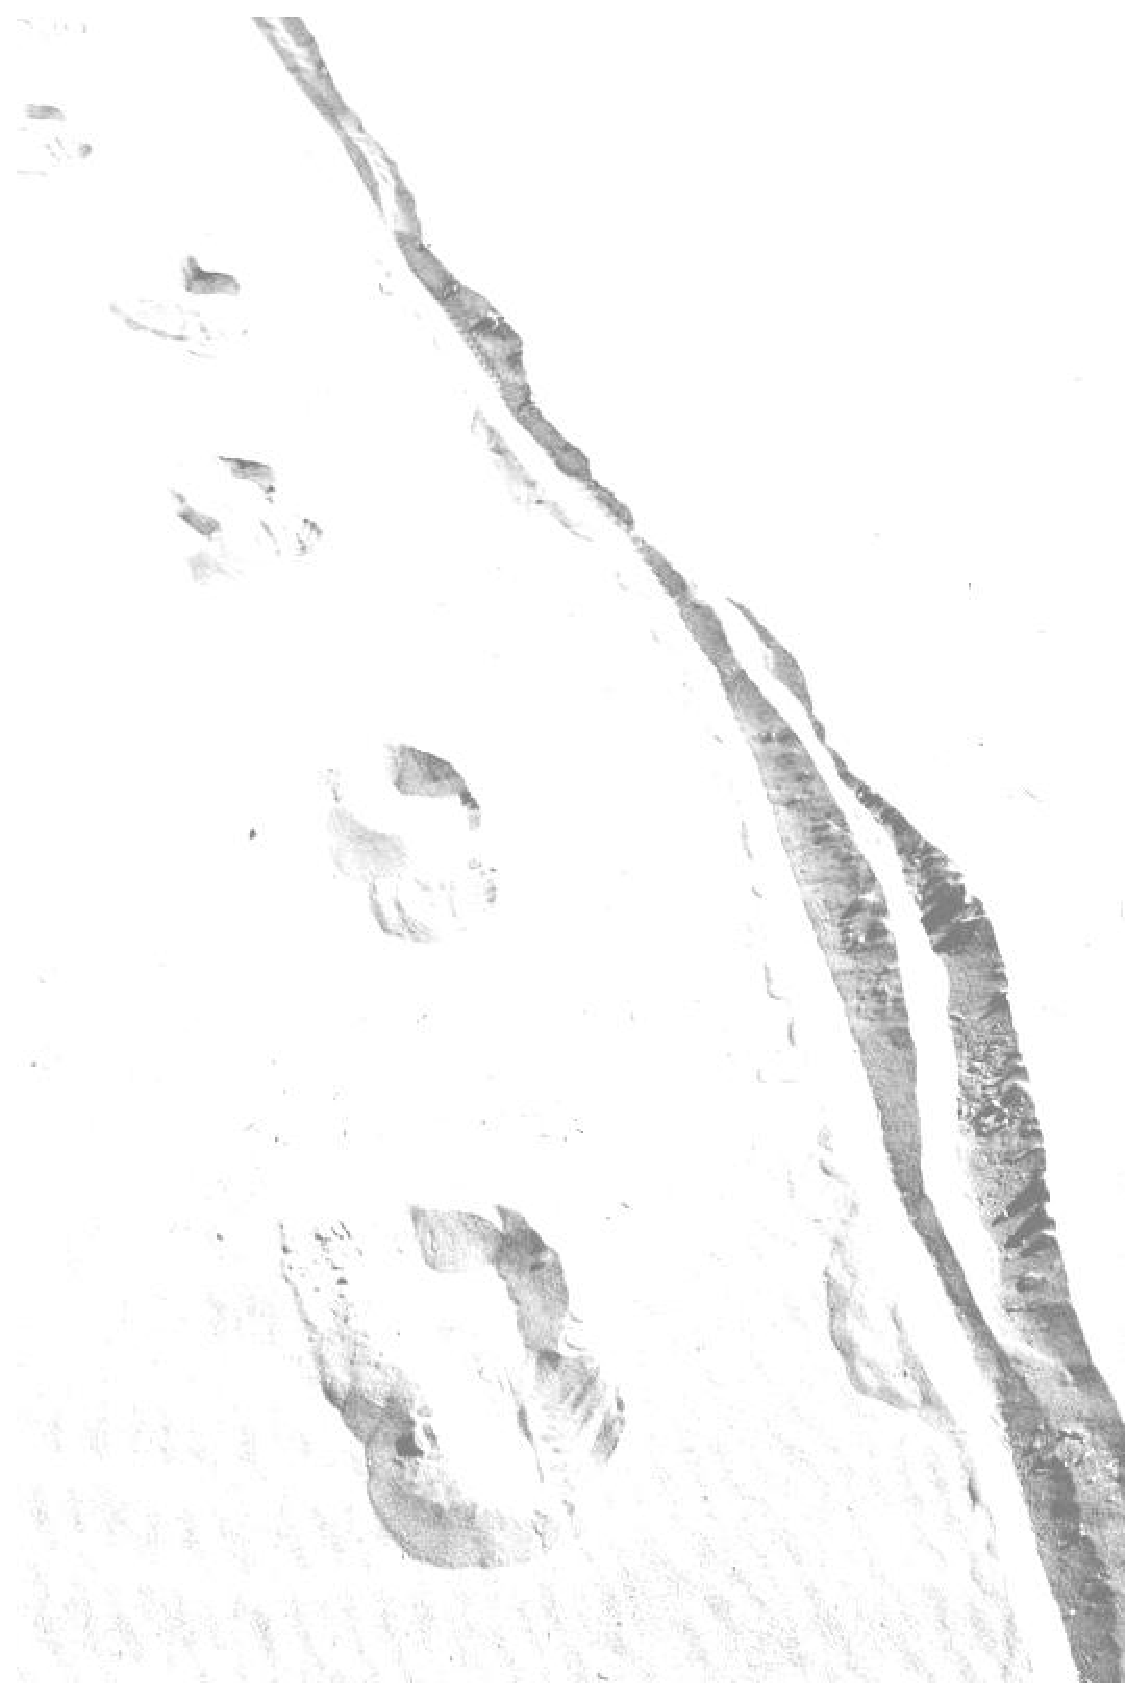
\includegraphics[width=0.55\paperwidth, height = \paperheight]{Figures/Track.eps}}}
  \begin{frame}{\normalsize Outline}
  \tableofcontents[currentsection]
  \end{frame}}
}



\title[Intro to Decisions]{Introduction to Theory of Safe Decision Making}
\author[???]{\large Dr. Akhil Anand}
%\institute[NTNU]{Prof. \\ Department of Cybernetic \\ Faculty of Information Technology \\  NTNU}
\date[September 2025]{$1^\mathrm{st}$ AID Scientific Workshop, Trondheim}

%%%%%%%%%%%%%%%%%%%%%%%%%%%%%%%%%%%%%%%%%%%%%%%%%%%%%%%%%%%%%%%%%%%%%%%%

\begin{document}







{\usebackgroundtemplate{
 \parbox[c][\paperheight][b]{\paperwidth}{
    \flushright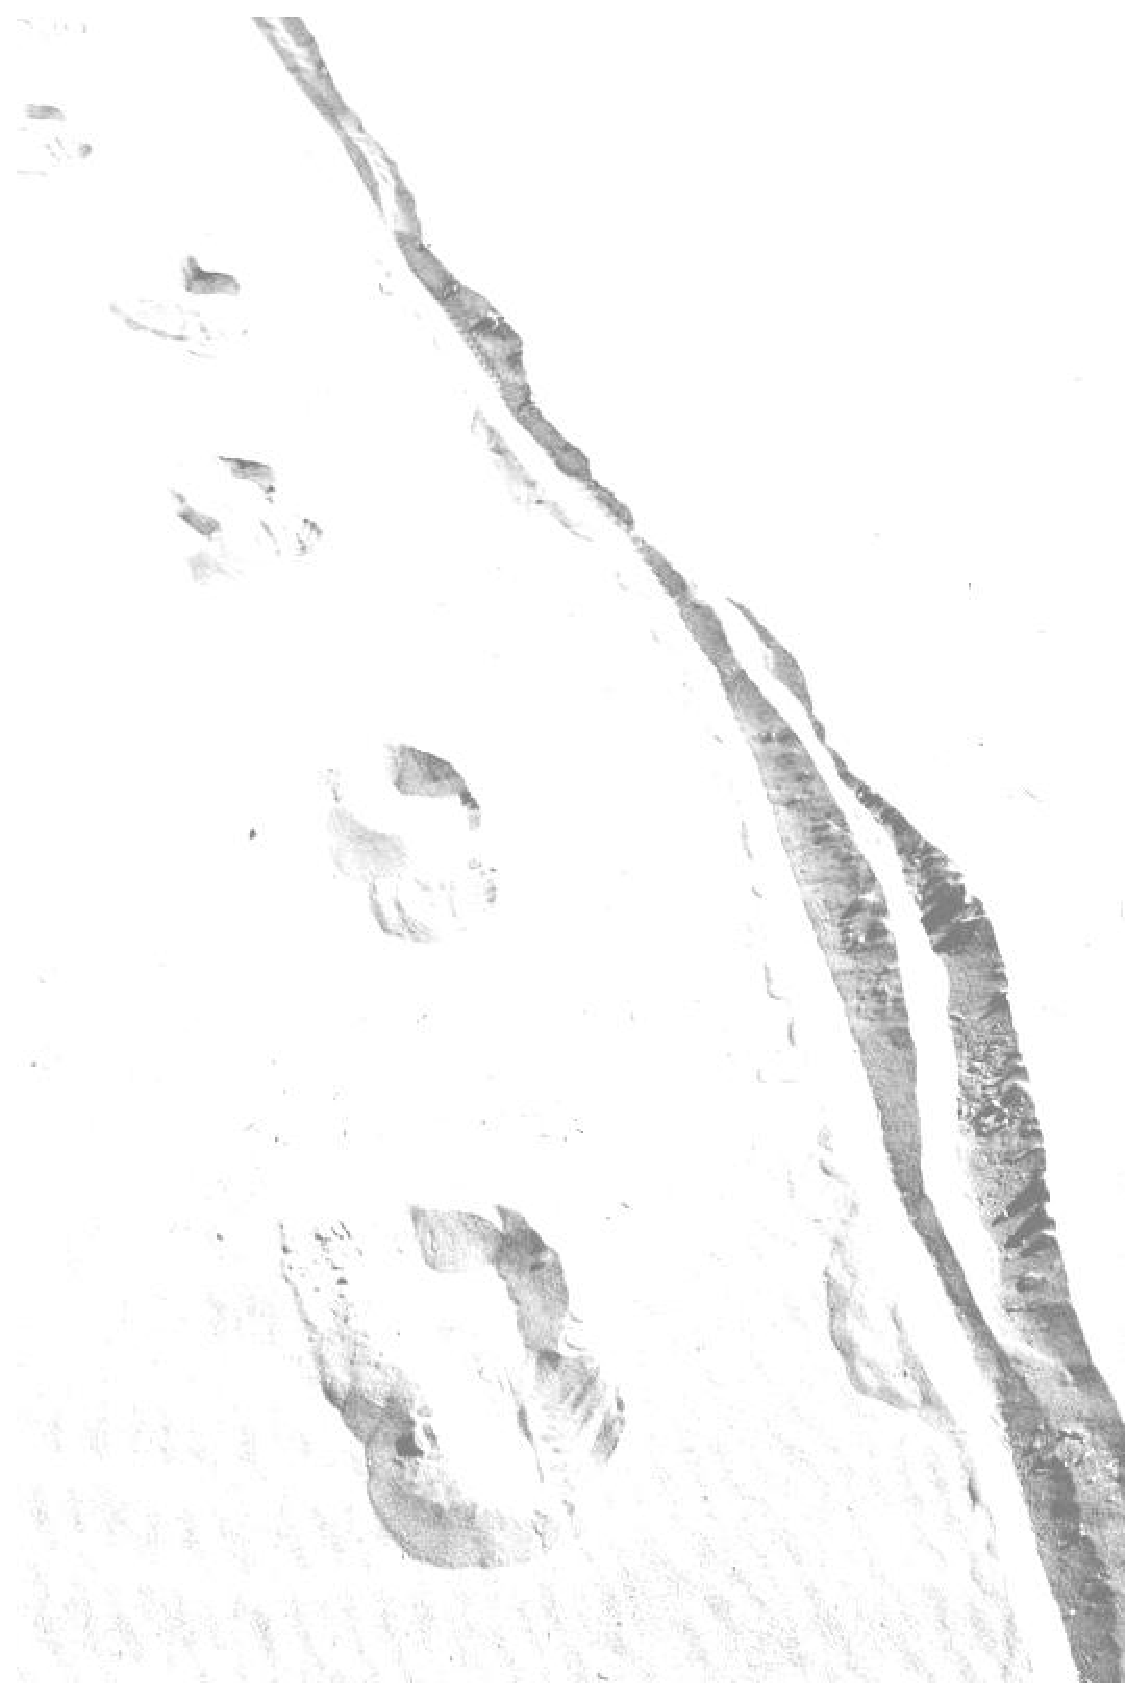
\includegraphics[width=0.55\paperwidth, height = 1\paperheight]{Figures/Track.eps}}}
\begin{frame}
\titlepage
\end{frame}}





\begin{frame}{\normalsize Forewords \& Disclaimer}
\footnotesize

\textbf{Objectives:}
\begin{itemize}
\item Put in place some common concepts \& language
\item Identify some key points in safe decision making 
\item Connect to AI
\end{itemize}
\center
\textbf{Disclaimer:} we are a broad group who needs to get to know each others scientifically. Apologies if I don't "hit" the right level for all. \\I have favored simplicity over ``absolute" rigor. 

\vspace{1cm}
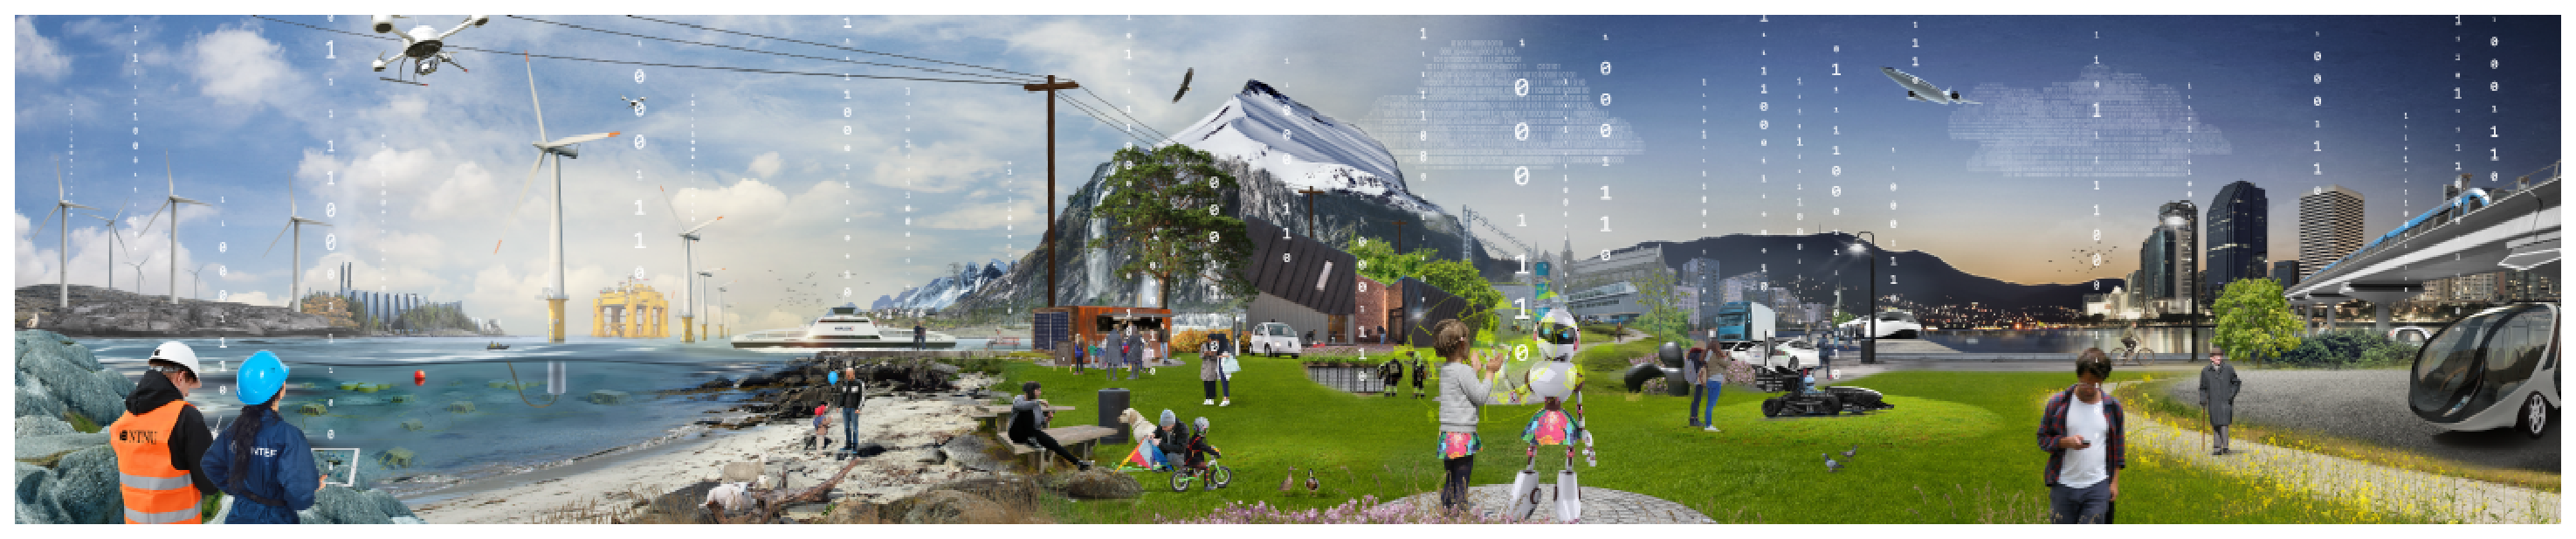
\includegraphics[width=1\textwidth,clip]{Figures/SmartGridLab.eps}

\end{frame}

\section{Some Basics of Safe Decision Making}


\begin{frame}{\normalsize Formally Defining Safety?}
\footnotesize

\newcommand{\Sys}{\vspace{-0.25cm}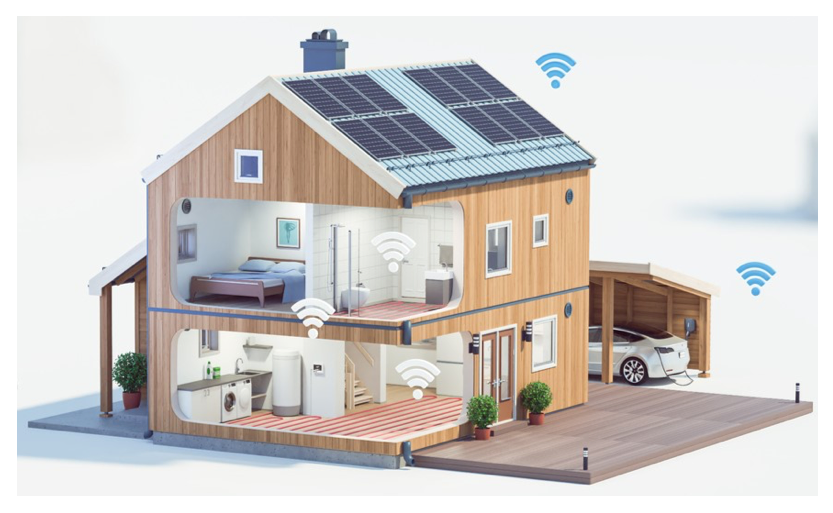
\includegraphics[width=1\textwidth,clip]{Figures/SmartHouse.eps}}

\tikzstyle{Sys_block} = [rectangle, draw, fill=none,  text width=3.cm, text centered, rounded corners, minimum height=4em,inner sep=2pt]
\tikzstyle{Opt_block} = [rectangle, draw, fill=myLightGreen,  text width=3.5cm,  text centered, rounded corners]
\tikzstyle{Util_block} = [rectangle, draw, fill=myLightBlue,  text width=3.5cm,  text centered, rounded corners]
\tikzstyle{Const_block} = [rectangle, draw, fill=myLightRed,  text width=3.5cm,  text centered, rounded corners]
\tikzstyle{line} = [draw, -latex']


\begin{tikzpicture}[->,>=stealth']

\node [Sys_block] (sys0) {\Sys};


 \node [Opt_block, left of=sys0, node distance = 5cm] (opt0) {
 \begin{minipage}[c]{3.5cm}
 \center
Information to Decisions\\
\textbf{Policy} $\vect\pi$
\end{minipage}
 };
 
  \node [Util_block, below of=opt0, node distance = 1.6cm] (util0) {
 \begin{minipage}[c]{3.5cm}
 \center
Utility
\end{minipage}
 };
  \node [Const_block, above of=opt0, node distance = 1.6cm] (limit0) {
 \begin{minipage}[c]{3.5cm}
 \center
Constraints
\end{minipage}
 };

 
 \path  (sys0) edge[bend left=20]  node[anchor=north] {Information} (opt0)
 (opt0) edge[bend left=20]  node[anchor=south] {Action} (sys0);
 \path (util0) edge[<->]  node[anchor=east] {Performance} (opt0);
\path (limit0) edge[<->]  node[anchor=east] {Violations} (opt0);
 
\end{tikzpicture}
\vspace{.25cm}
\begin{columns}[t]
\column{0.35\textwidth}
%\center
\textbf{Safety in the real world}
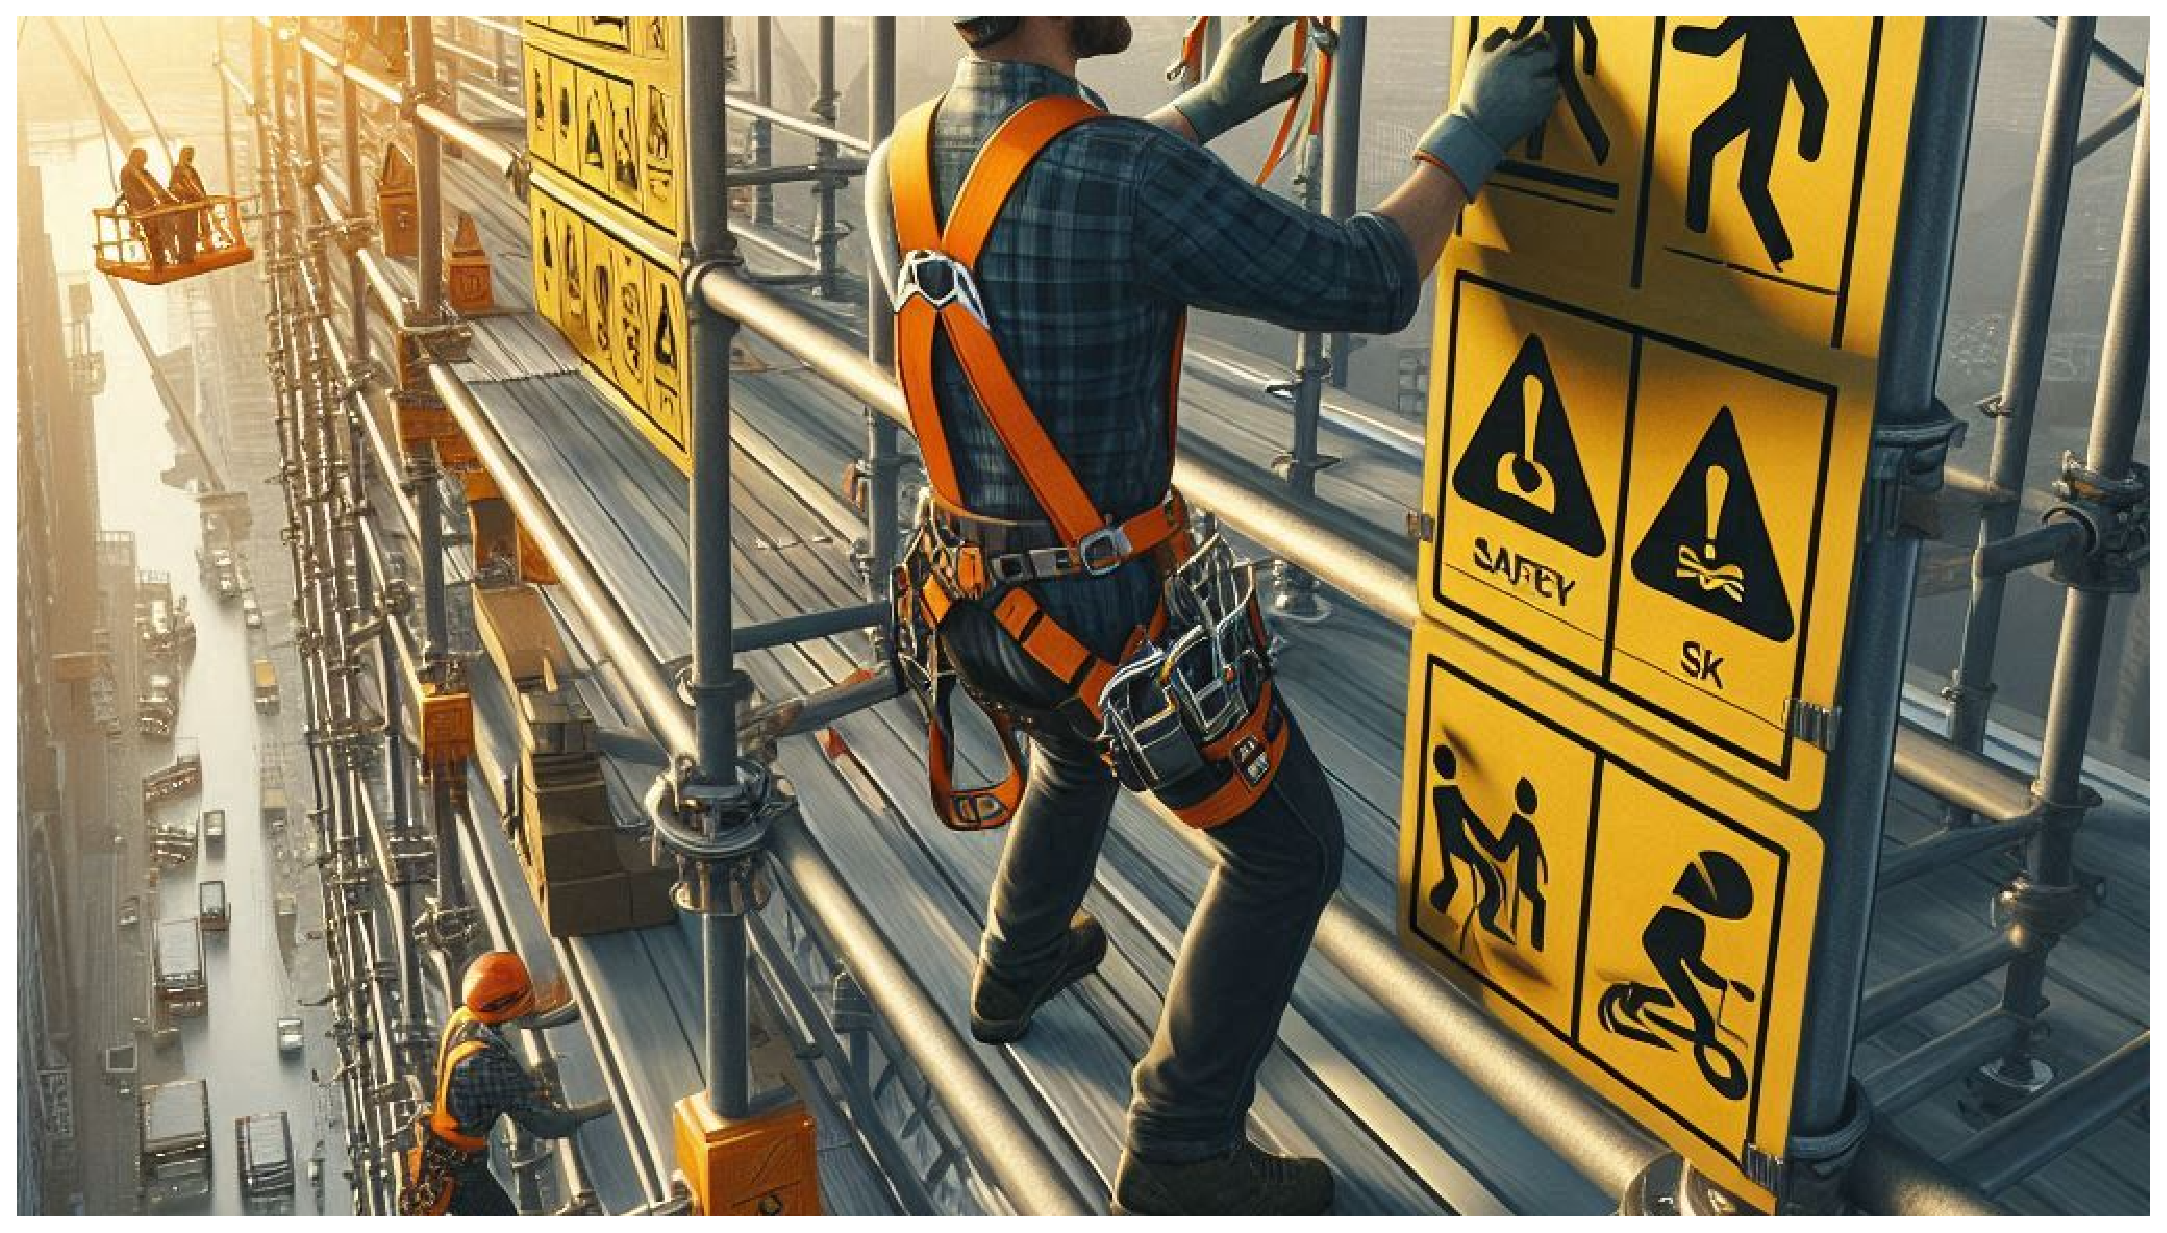
\includegraphics[width=1\textwidth,clip]{Figures/OSHA.eps}
\column{0.2\textwidth}
\vspace{.1cm}
%\center
%\includegraphics[width=1\textwidth,clip]{Figures/Bridge.eps}

\includegraphics[width=1\textwidth,clip,angle=-15]{Figures/Arrow.eps}
\column{0.45\textwidth}
%\center
\textbf{Safety in the math world} \\ %Stay within certain ``sets"
\vspace{-.25cm}
  \begin{overlayarea}{\textwidth}{0.3\textheight}
    \begin{figure}
     \newcommand{\FS}{0.7}

      \only<1-3>
        {%
       \hspace{-1.5cm}   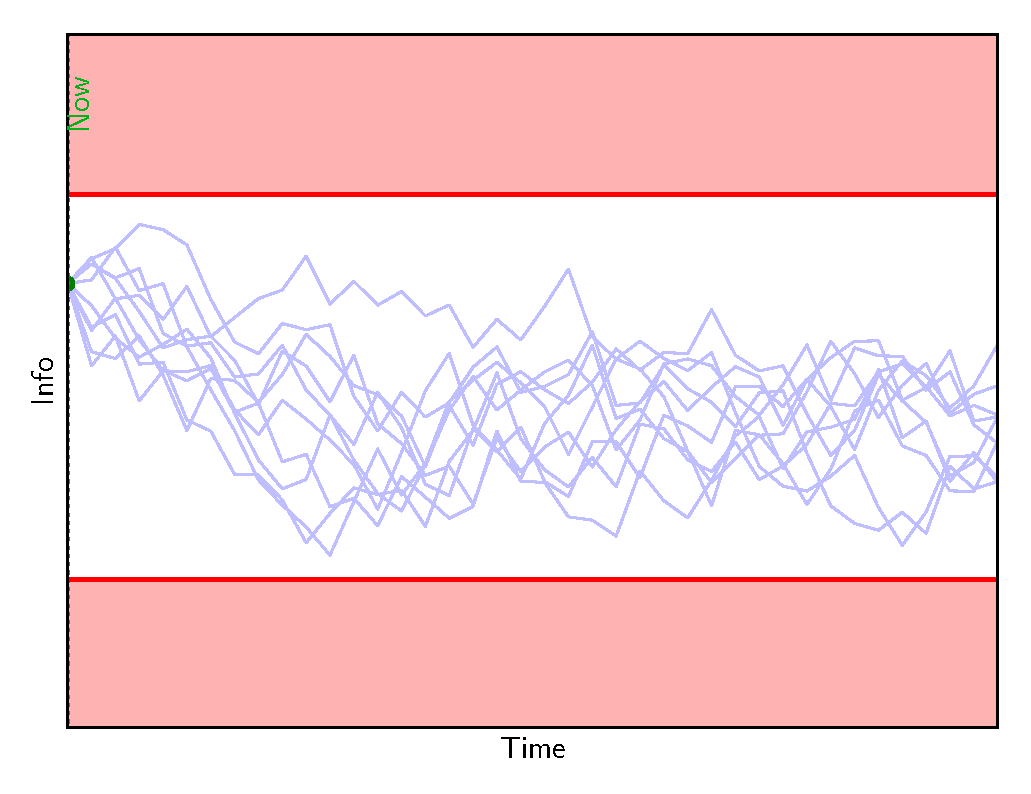
\includegraphics[width=\FS\textwidth]{Codes/BasicsSafety/Safe0.eps}%
        }%
              \only<4>
        {%
        \hspace{-1.5cm}            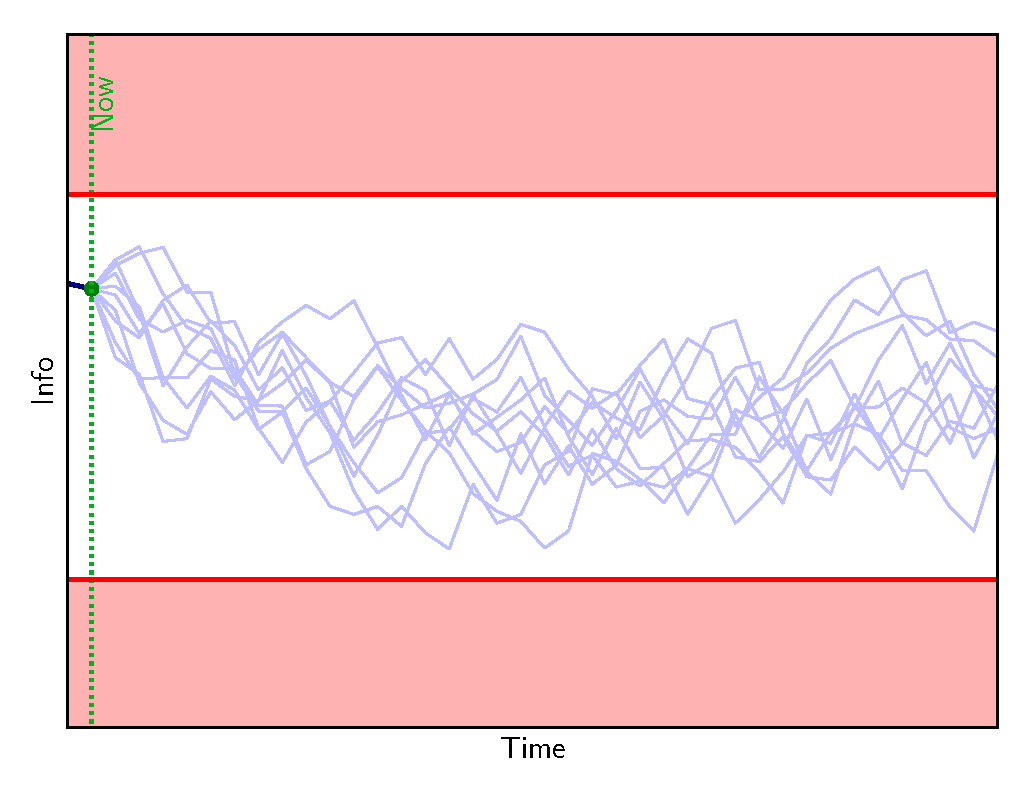
\includegraphics[width=\FS\textwidth]{Codes/BasicsSafety/Safe1.eps}%
        }%
                      \only<5>
        {%
       \hspace{-1.5cm}             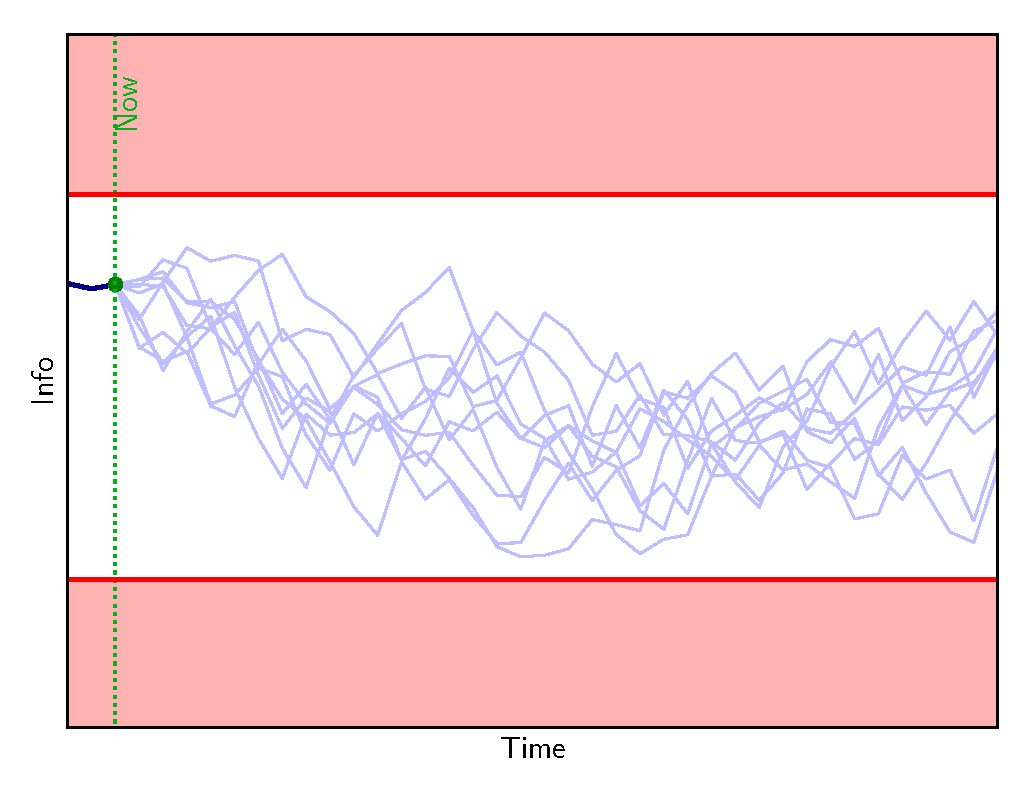
\includegraphics[width=\FS\textwidth]{Codes/BasicsSafety/Safe2.eps}%
        }%
                      \only<6>
        {%
       \hspace{-1.5cm}             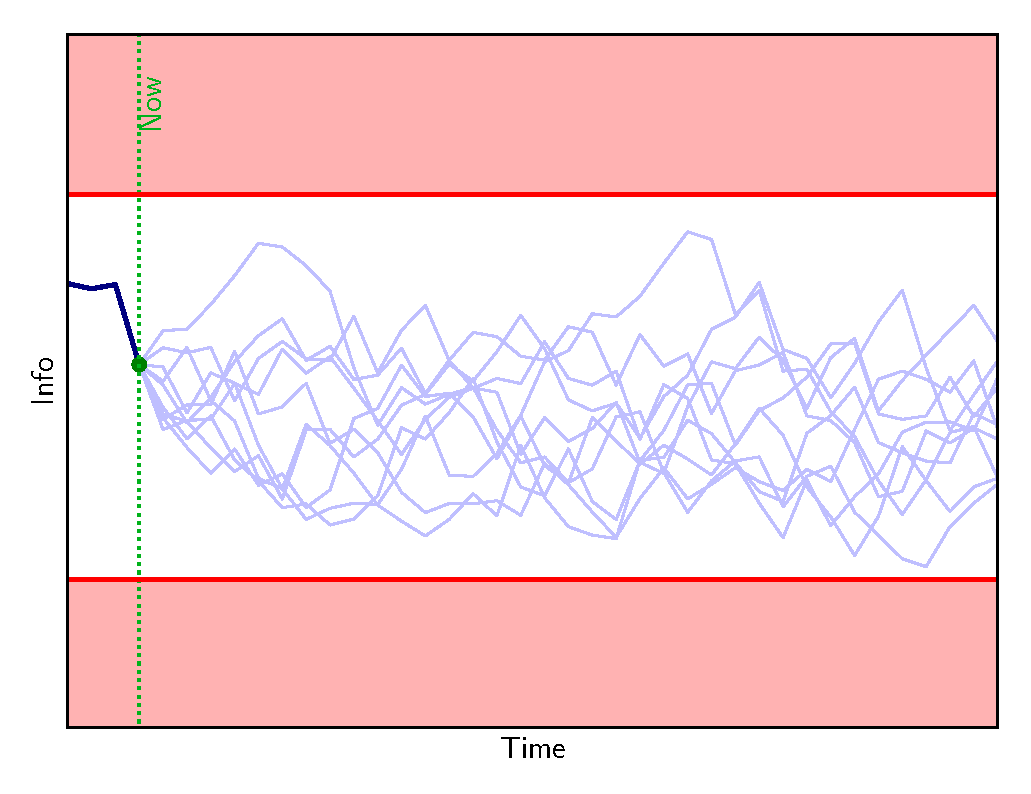
\includegraphics[width=\FS\textwidth]{Codes/BasicsSafety/Safe3.eps}%
        }%
                      \only<7>
        {%
       \hspace{-1.5cm}             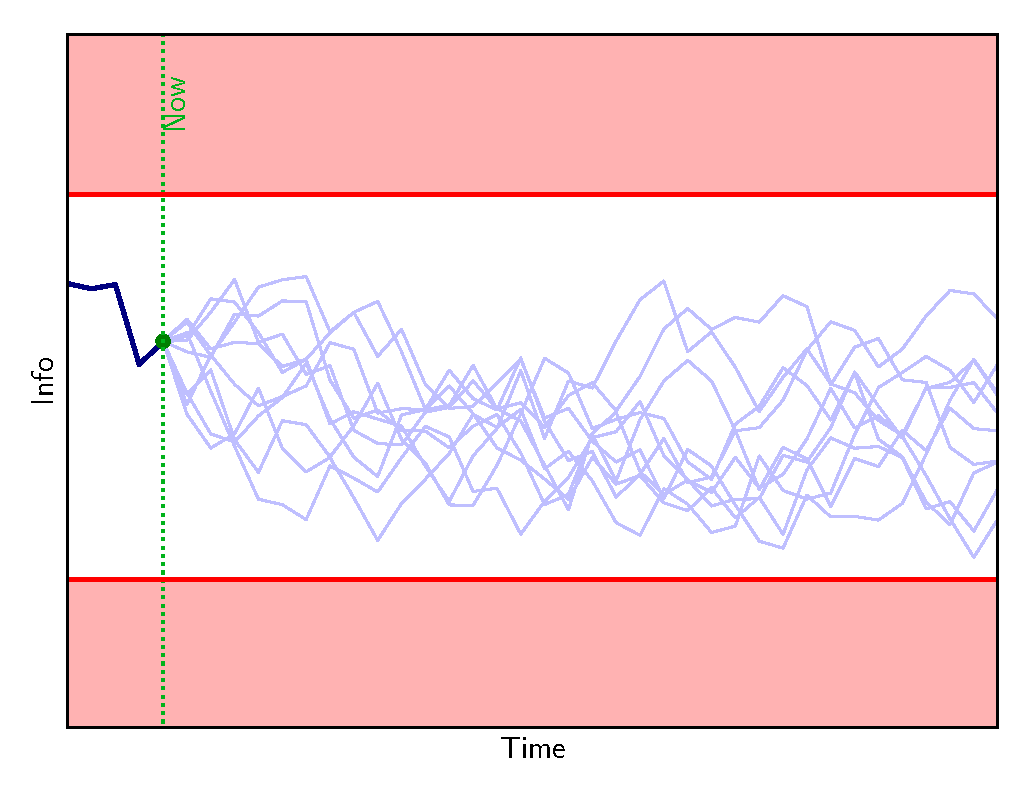
\includegraphics[width=\FS\textwidth]{Codes/BasicsSafety/Safe4.eps}%
        }%
                      \only<8>
        {%
       \hspace{-1.5cm}             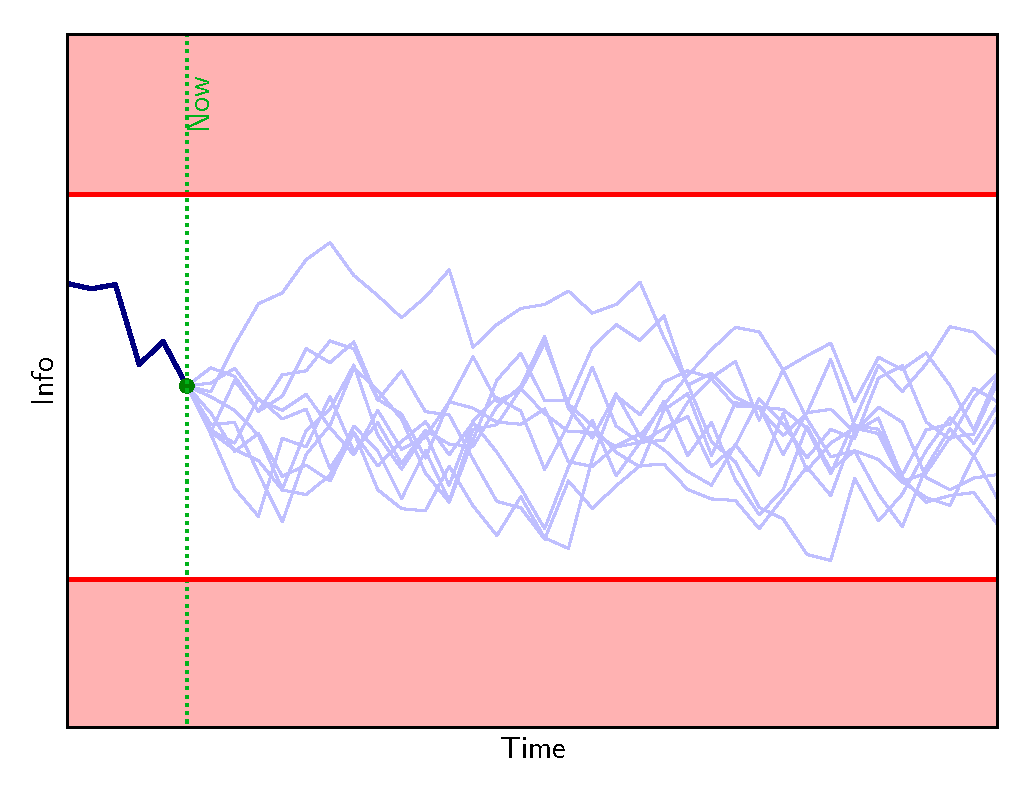
\includegraphics[width=\FS\textwidth]{Codes/BasicsSafety/Safe5.eps}%
        }%
                      \only<9>
        {%
       \hspace{-1.5cm}             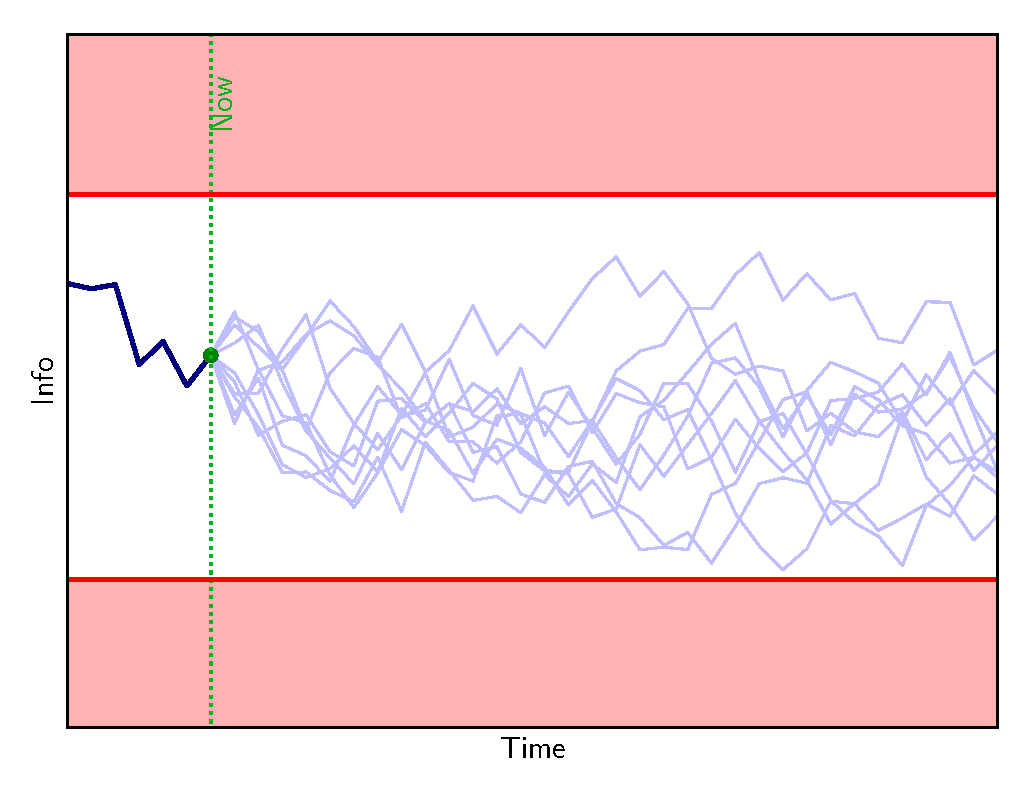
\includegraphics[width=\FS\textwidth]{Codes/BasicsSafety/Safe6.eps}%
        }%
                      \only<10>
        {%
       \hspace{-1.5cm}             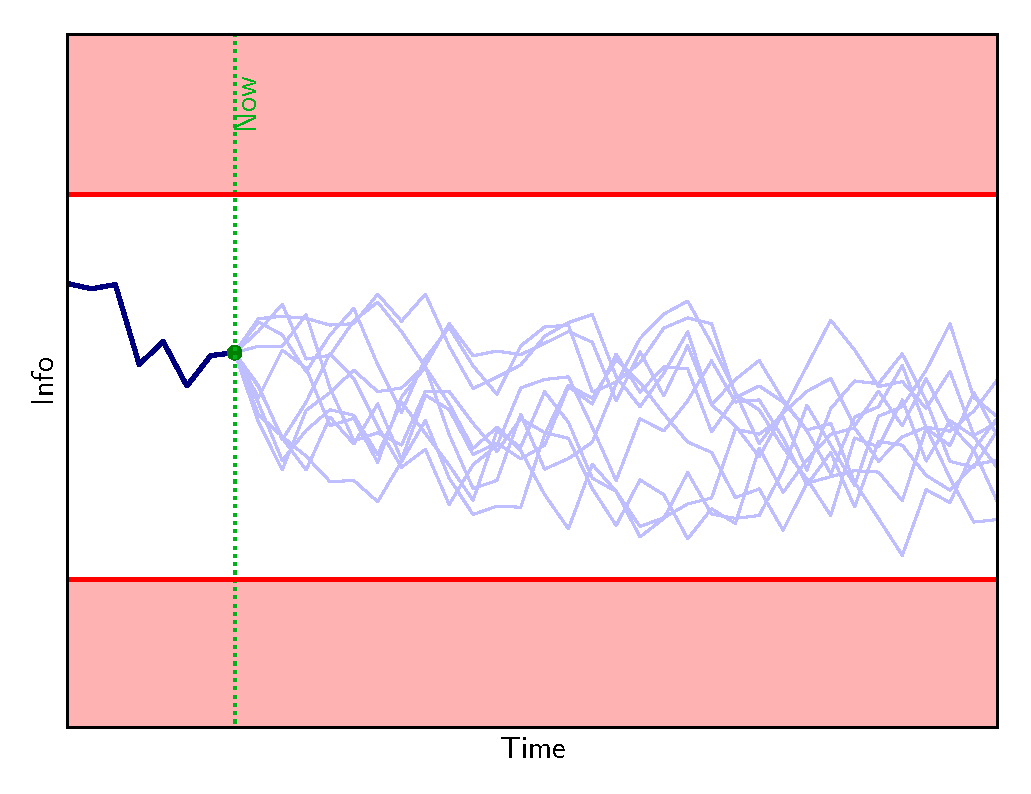
\includegraphics[width=\FS\textwidth]{Codes/BasicsSafety/Safe7.eps}%
        }%
    \end{figure}
  \end{overlayarea} 
  
  
  

\end{columns}

\end{frame}

%\section{Safe Decision Making}

\begin{frame}{\normalsize Constrained MDPs}
\footnotesize
\vspace{-0.5cm}
\begin{columns}
\column{0.5\textwidth}
\begin{alertblock}{}
\textbf{In words}
\vspace{-.25cm}
\begin{align*}
\vect\pi^\star = \argmax_{\vect\pi}&\quad\mathrm E\left[ \sum_{\text{time}} \text{Utility}\right]\\
\mathrm{s.t.}&\quad \text{Constraints ok at all time}
\end{align*}
\end{alertblock}
\column{0.3\textwidth}
 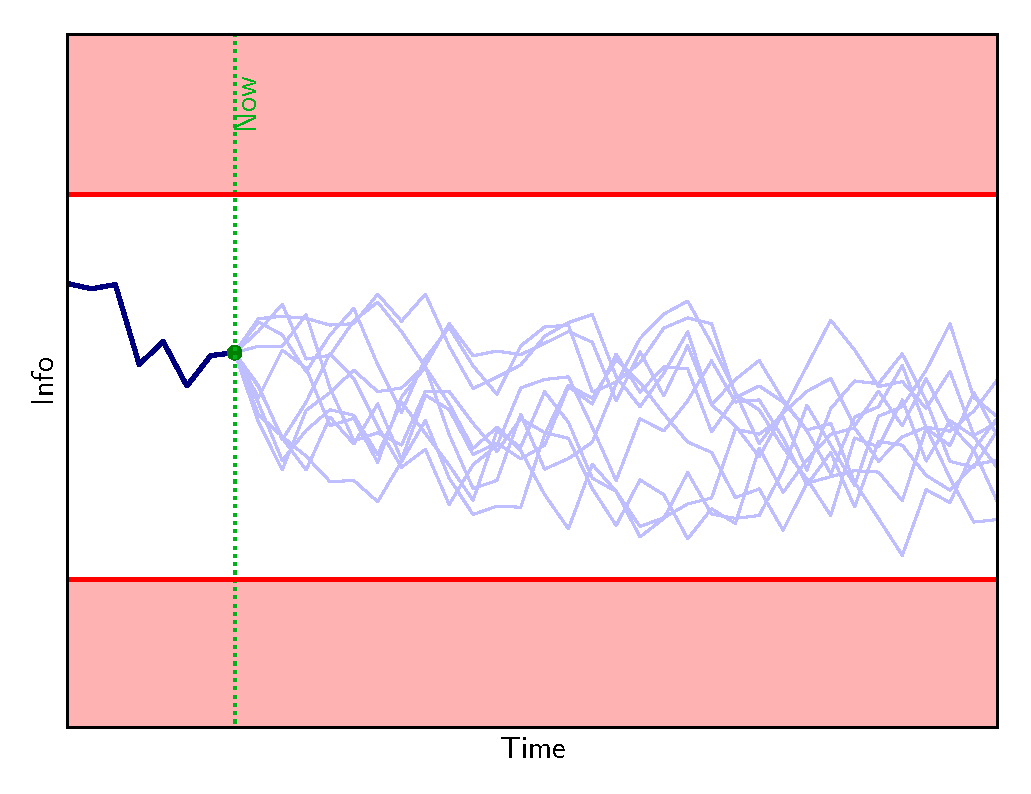
\includegraphics[width=1\textwidth]{Codes/BasicsSafety/Safe7.eps}
\end{columns}
\visible<2->{
\begin{block}{}
\textbf{Formally}
\vspace{-.25cm}
\begin{align*}
\vect\pi^\star = \argmax_{\vect\pi}&\quad\mathrm E\left[  \sum_{\text{time}} \left(\text{Utility} - \cmatr{ccc}{0&\text{if}&\text{Constraint ok}\\\infty &\text{if}&\text{Constraint not ok}}\right)\right]
\end{align*}
\end{block}}
%\visible<3->{
%\textbf{Remarks}: $-\infty$ penalty on constraints violations $\Rightarrow$ safe policy (mathematically) } \underline{but}
%\begin{columns}
%\column{0.6\textwidth}
\visible<3->{\textbf{Build policy} using
\begin{itemize}
\item Perfect model of the real world $\hat{\mathrm P}[\vect s_+|\vect s,\vect a]=\mathrm P[\vect s_+|\vect s,\vect a]$
\item Model ``pessimistic" about the uncertainties
%\item \visible<4->{Formally support of $\mathrm P[\cdot|\vect s,\vect a]$ is included in  support of $\hat{\mathrm P}[\cdot|\vect s,\vect a]$}
\end{itemize}
... to evaluate ``$\mathrm E[\cdot]$"
}

%\column{0.4\textwidth}
%\hspace{-2cm}\includegraphics[width=1.5\textwidth,clip]{Codes/BasicsSafety/PessimisticOneStep.eps}
%\end{columns}

%\begin{columns}
%\column{0.5\textwidth}
%\visible<3->{
%\begin{itemize}
%\item Requires perfect (or pessimistic) model 
%\item Perfect (or pessimistic) policy calculation 
%\item Pessimistic? In case of doubt, assume the worst...
%\end{itemize}}
%\center
%\visible<4->{\textcolor{myBlue2}{\textbf{Classical view:\\ ``Robust" decision making}}}
%\column{0.5\textwidth}
%\vspace{-1cm}
%  \begin{overlayarea}{\textwidth}{0.4\textheight}
%    \begin{figure}
%     \newcommand{\FS}{0.65}
%      \only<3>
%        {%
%       \hspace{-1.5cm}   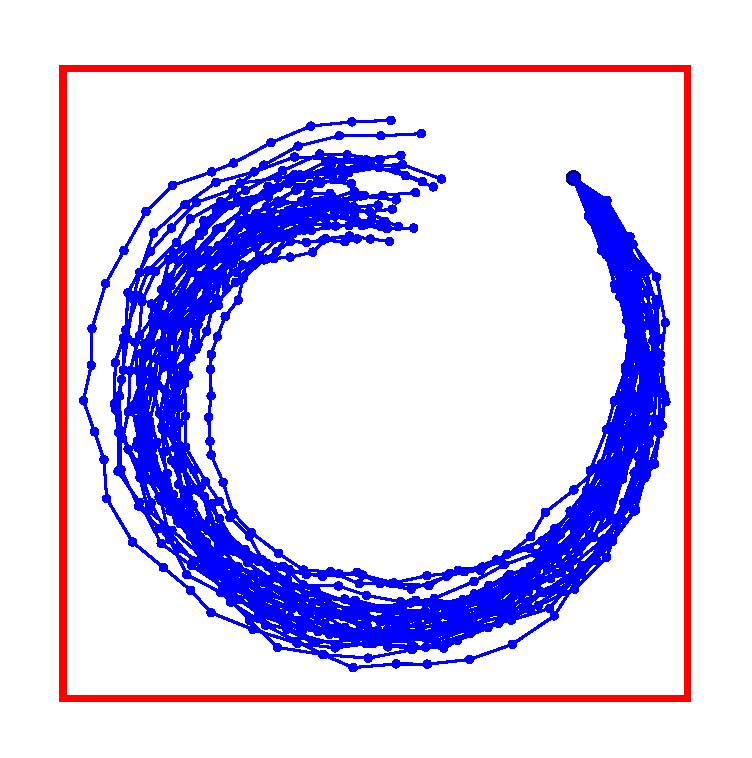
\includegraphics[width=\FS\textwidth]{Codes/BasicsSafety/PessimisticModelSTEPBOXED0.eps}%
%        }%
%              \only<4>
%        {%
%       \hspace{-1.5cm}   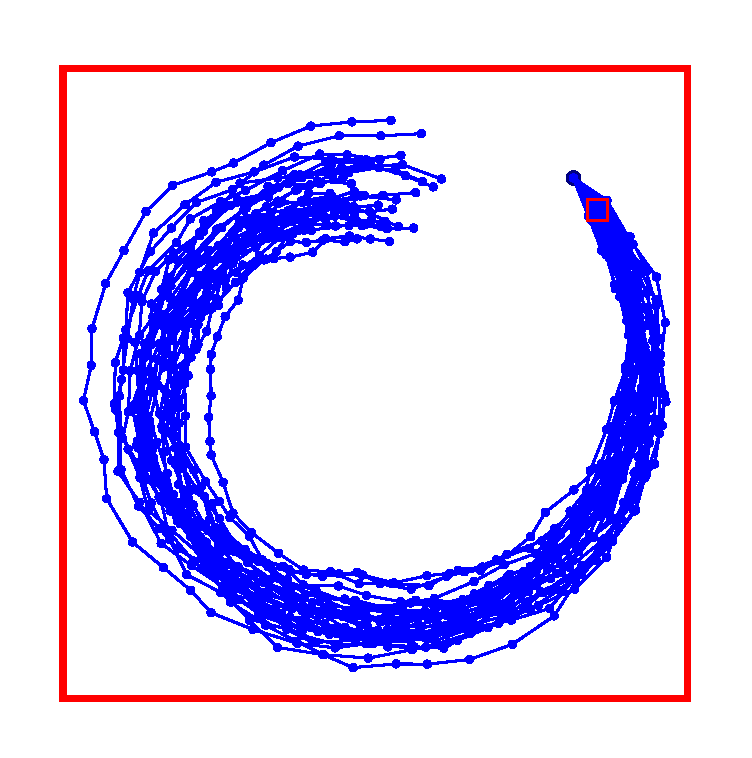
\includegraphics[width=\FS\textwidth]{Codes/BasicsSafety/PessimisticModelSTEPBOXED1.eps}%
%        }%
%              \only<5>
%        {%
%       \hspace{-1.5cm}   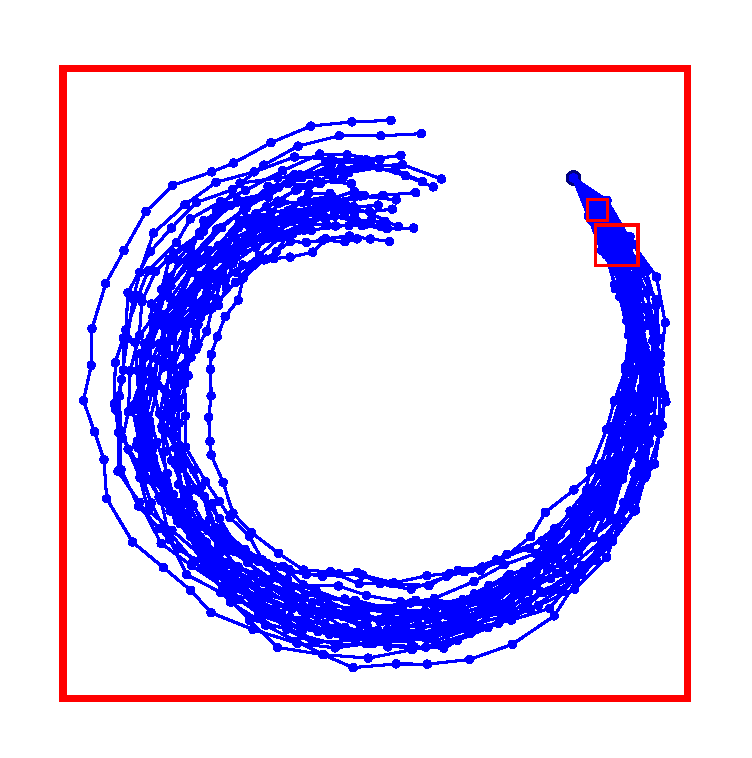
\includegraphics[width=\FS\textwidth]{Codes/BasicsSafety/PessimisticModelSTEPBOXED2.eps}%
%        }%
%                      \only<6>
%        {%
%       \hspace{-1.5cm}   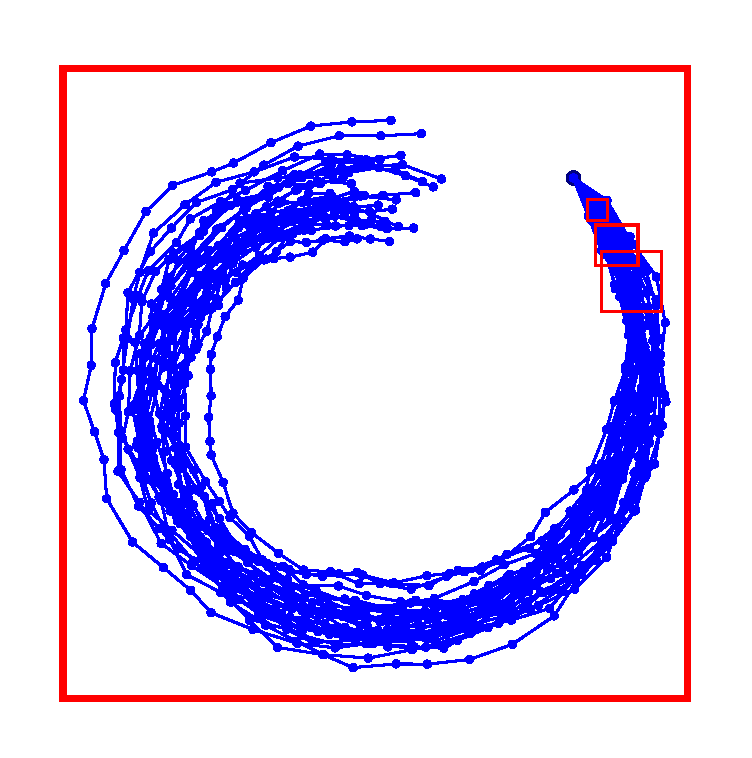
\includegraphics[width=\FS\textwidth]{Codes/BasicsSafety/PessimisticModelSTEPBOXED3.eps}%
%        }%
%                      \only<7>
%        {%
%       \hspace{-1.5cm}   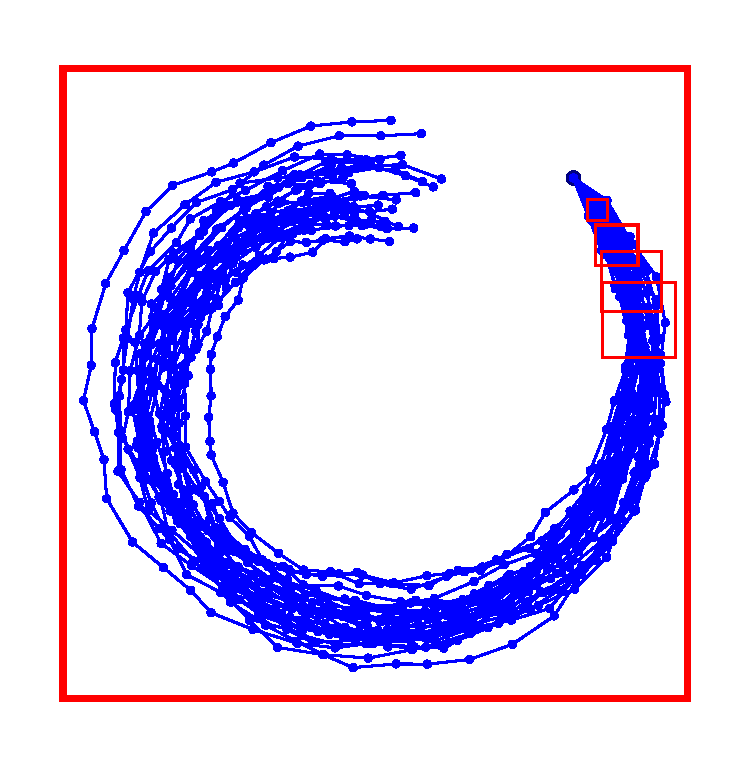
\includegraphics[width=\FS\textwidth]{Codes/BasicsSafety/PessimisticModelSTEPBOXED4.eps}%
%        }%
%                              \only<8>
%        {%
%       \hspace{-1.5cm}   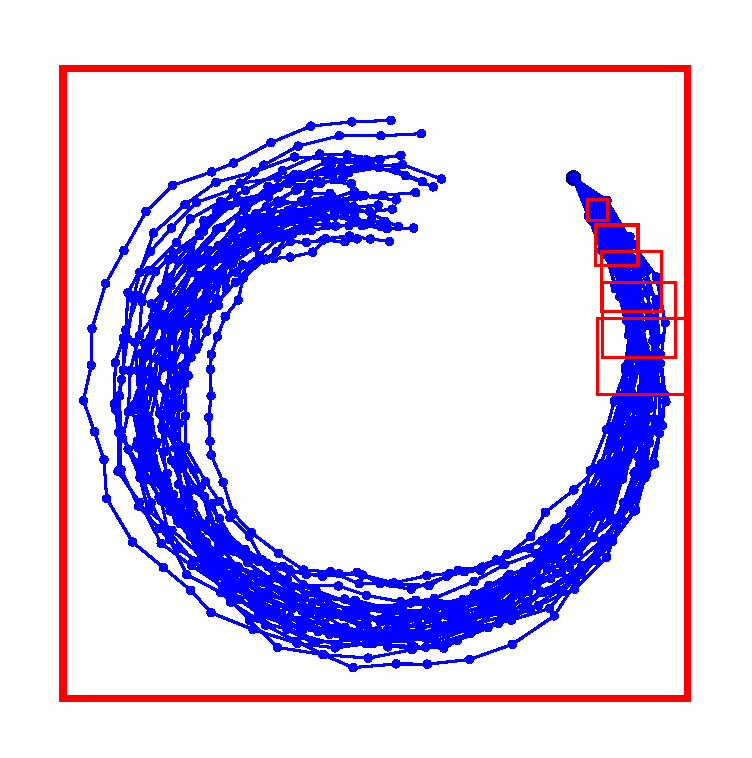
\includegraphics[width=\FS\textwidth]{Codes/BasicsSafety/PessimisticModelSTEPBOXED5.eps}%
%        }%
%                              \only<9>
%        {%
%       \hspace{-1.5cm}   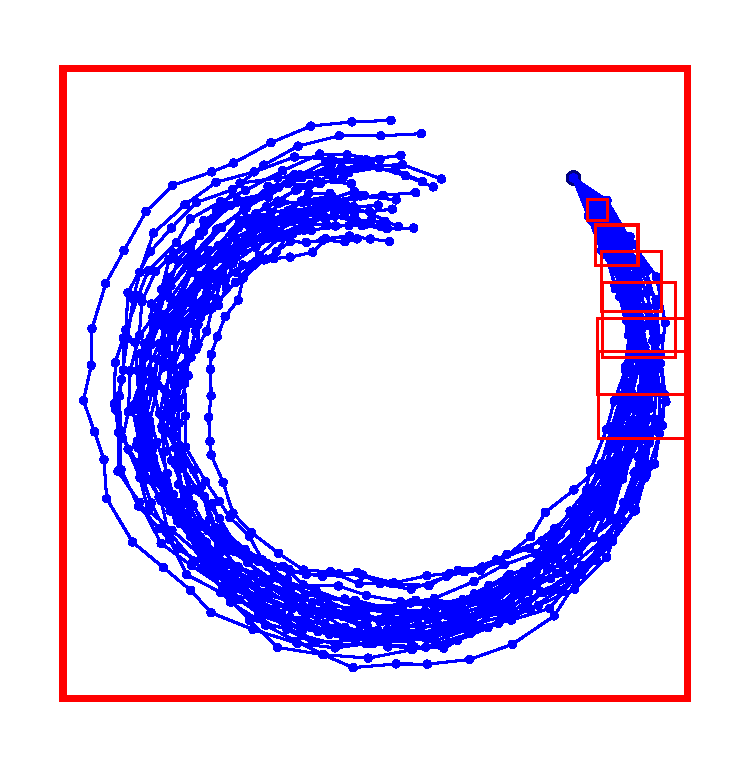
\includegraphics[width=\FS\textwidth]{Codes/BasicsSafety/PessimisticModelSTEPBOXED6.eps}%
%        }%
%                              \only<10>
%        {%
%       \hspace{-1.5cm}   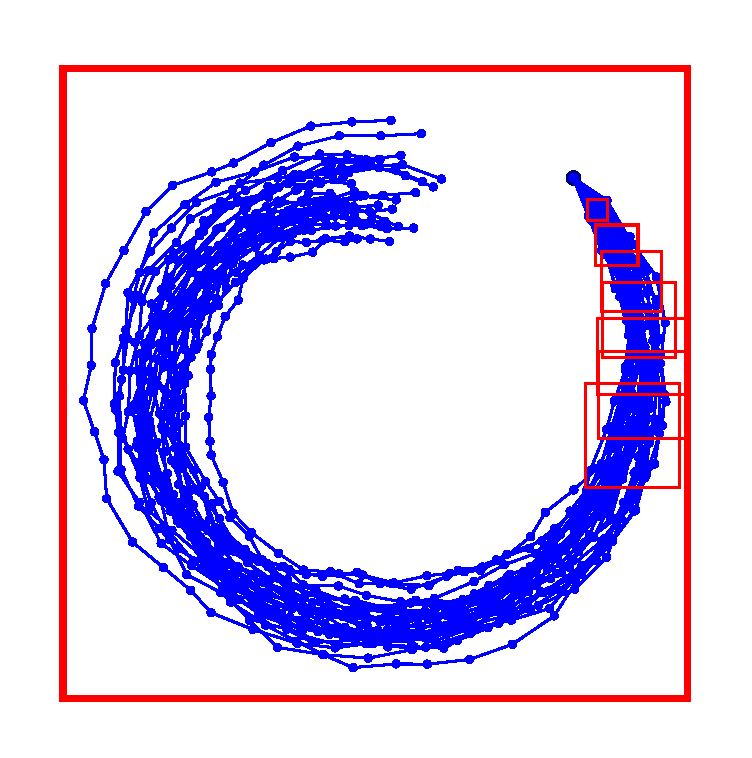
\includegraphics[width=\FS\textwidth]{Codes/BasicsSafety/PessimisticModelSTEPBOXED7.eps}%
%        }%
%                      \only<11->
%        {%
%       \hspace{-1.5cm}   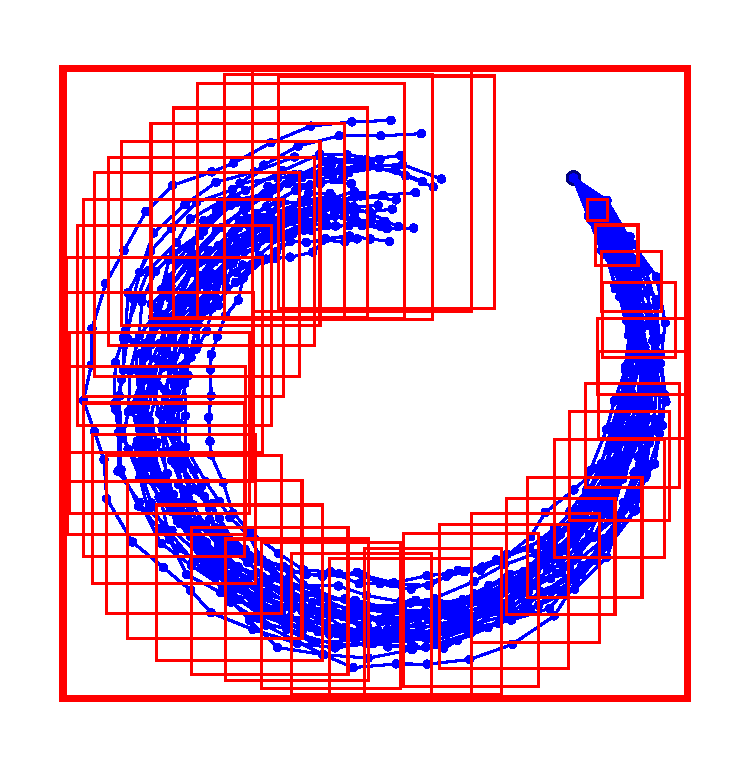
\includegraphics[width=\FS\textwidth]{Codes/BasicsSafety/PessimisticModelSTEPBOXED40.eps}%
%        }%
%    \end{figure}
%  \end{overlayarea} 
%  
%
%\end{columns}

\end{frame}


\begin{frame}{\normalsize Pessimistic Models for Decision Making}
\footnotesize
\begin{columns}[t]
\column{0.6\textwidth}
\begin{itemize}
\item Model must ``contain" the uncertainty 
\item ``Container" (set) should be simple for computational reasons
\item Trajectories predicted by pessimistic model will ``cover" the real world
\item Decision policy wants to be safe w.r.t. the ``containers"
\end{itemize}
\vspace{0.5cm}
\visible<12->{
\textbf{Remarks}
\begin{itemize}
\item The propagation of the ``containers" in the model predictions can be expensive / difficult
\item Pessimistic propagations are usually needed $\rightarrow$ pessimistic over pessimistic
\item Policy based on worst-case perspective makes the decisions highly conservative
\item Often labelled ``Robust" decision making
\end{itemize}
}


\column{0.4\textwidth}


  \begin{overlayarea}{\textwidth}{1\textheight}
    \begin{figure}
     \newcommand{\FS}{1}
      \only<1>
        {
        \center
        Distribution of one-step forward
	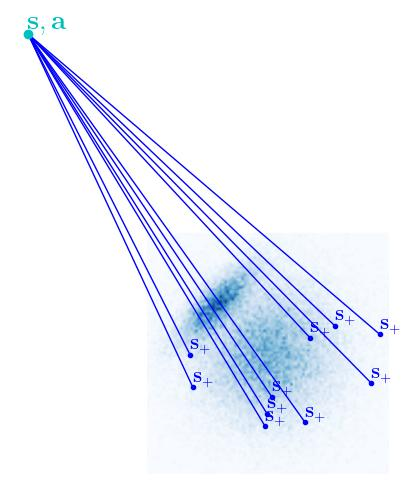
\includegraphics[width=1\textwidth,clip]{Codes/BasicsSafety/PessimisticOneStep0.eps}
	}
      \only<2>
        {
        \center
        Distribution of one-step forward with ``container"
	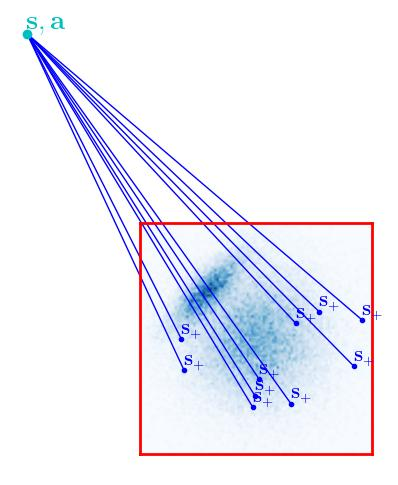
\includegraphics[width=1\textwidth,clip]{Codes/BasicsSafety/PessimisticOneStep1.eps}
	}
      \only<3>
        {%
        \center
        Trajectories 
   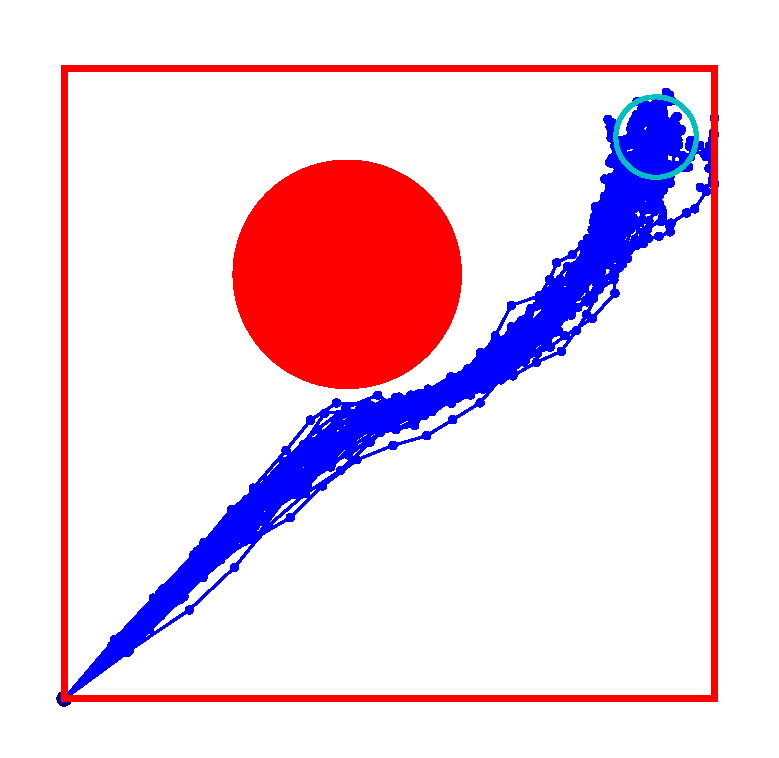
\includegraphics[width=\FS\textwidth]{Codes/BasicsSafety/PessimisticModel0.eps}%
        }%
              \only<4>
        {%
        \center
        Trajectories with ``containers"
  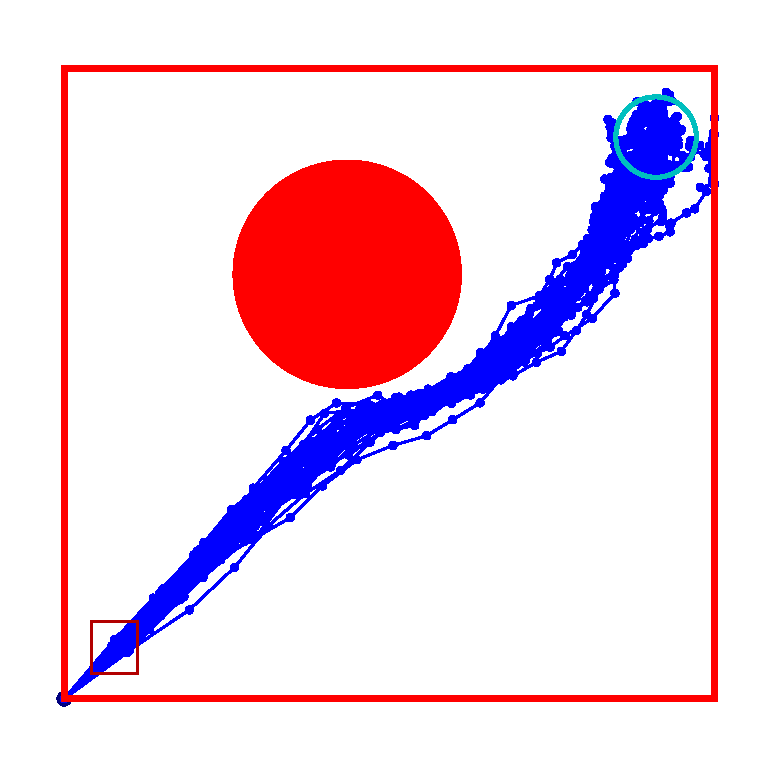
\includegraphics[width=\FS\textwidth]{Codes/BasicsSafety/PessimisticModel1.eps}%
        }%
              \only<5>
        {%
                \center
        Trajectories with ``containers"
  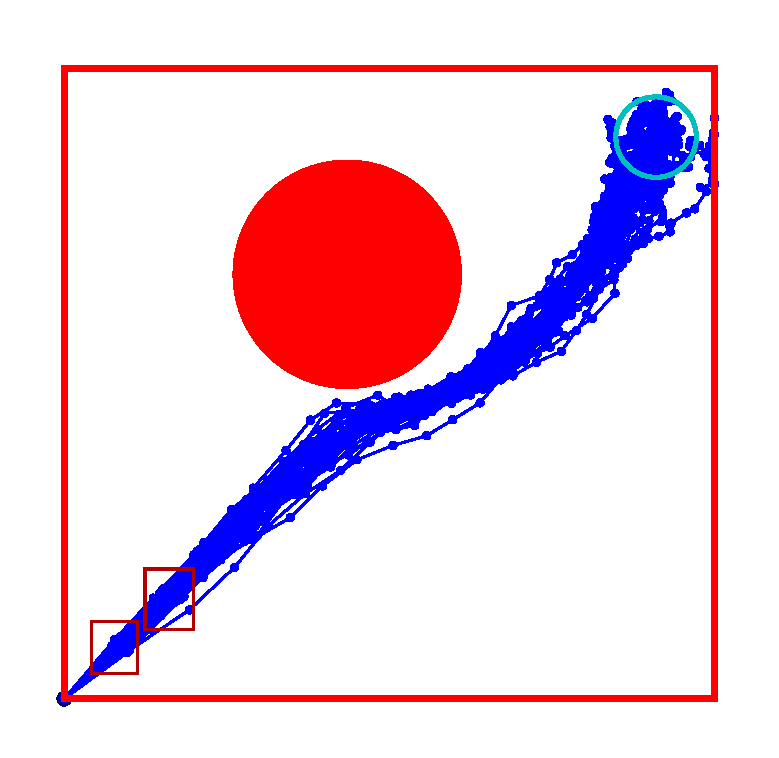
\includegraphics[width=\FS\textwidth]{Codes/BasicsSafety/PessimisticModel2.eps}%
        }%
                      \only<6>
        {%
                \center
        Trajectories with ``containers"
  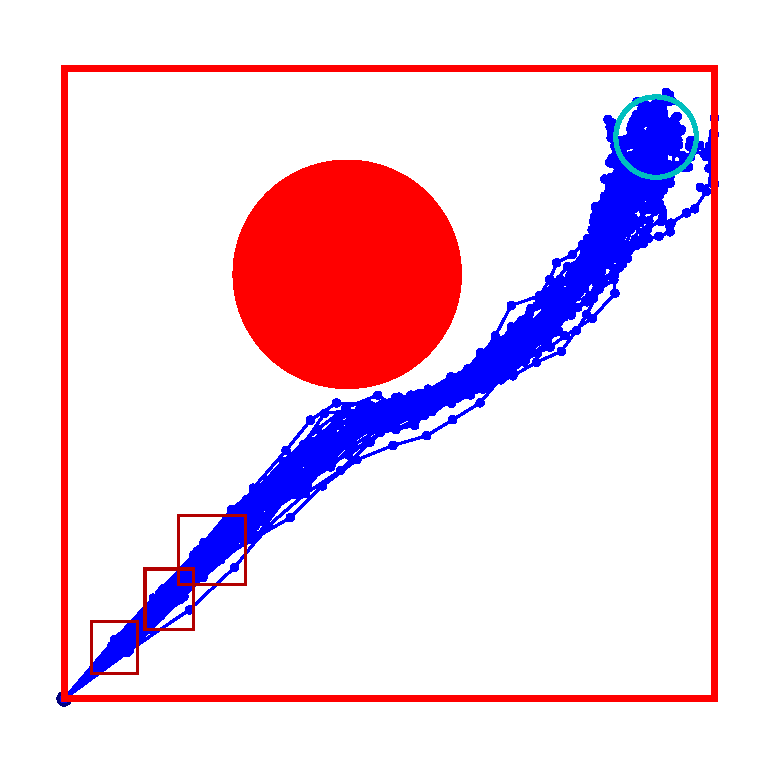
\includegraphics[width=\FS\textwidth]{Codes/BasicsSafety/PessimisticModel3.eps}%
        }%
                      \only<7>
        {%
                \center
        Trajectories with ``containers"
   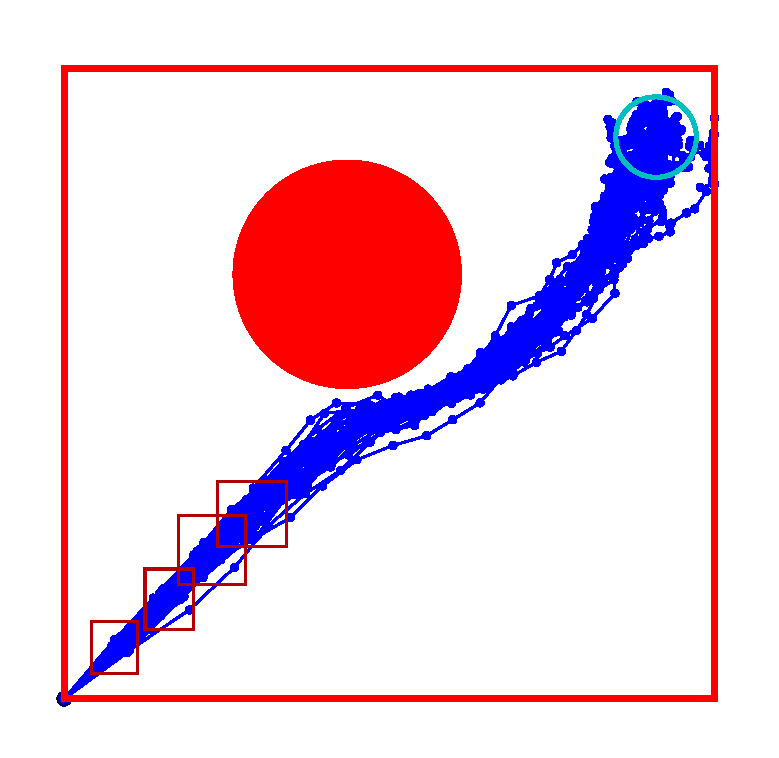
\includegraphics[width=\FS\textwidth]{Codes/BasicsSafety/PessimisticModel4.eps}%
        }%
                              \only<8>
        {%
                \center
        Trajectories with ``containers"
  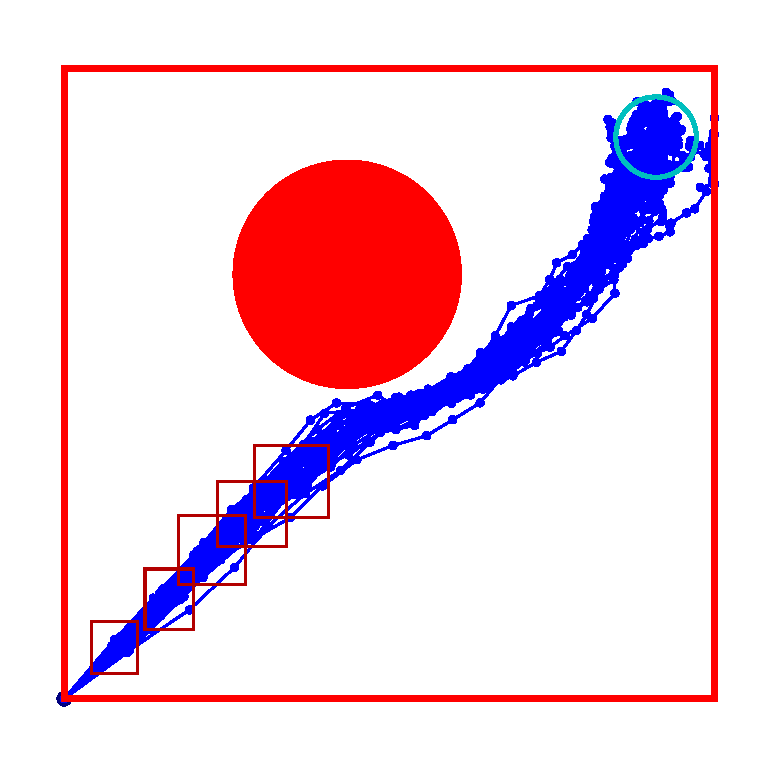
\includegraphics[width=\FS\textwidth]{Codes/BasicsSafety/PessimisticModel5.eps}%
        }%
                              \only<9>
        {%
                \center
        Trajectories with ``containers"
   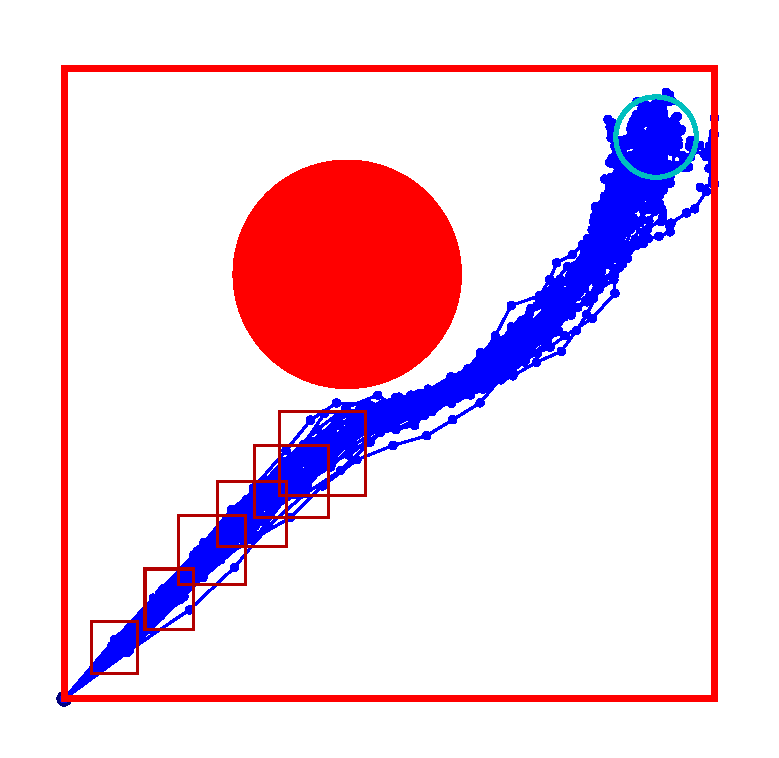
\includegraphics[width=\FS\textwidth]{Codes/BasicsSafety/PessimisticModel6.eps}%
        }%
                              \only<10>
        {%
                \center
        Trajectories with ``containers"
  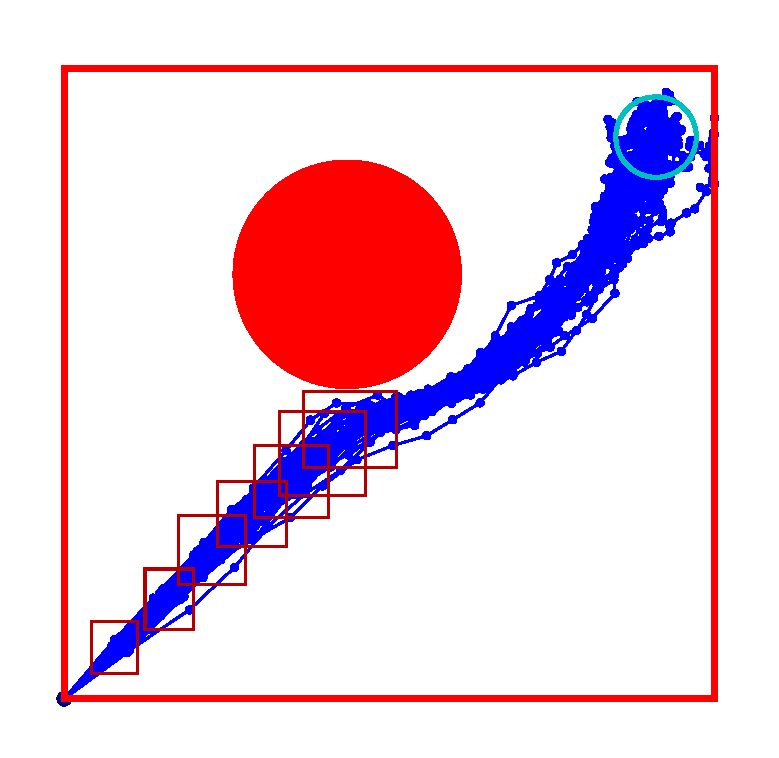
\includegraphics[width=\FS\textwidth]{Codes/BasicsSafety/PessimisticModel7.eps}%
        }%
                      \only<11->
        {%
                \center
        Trajectories with ``containers"
   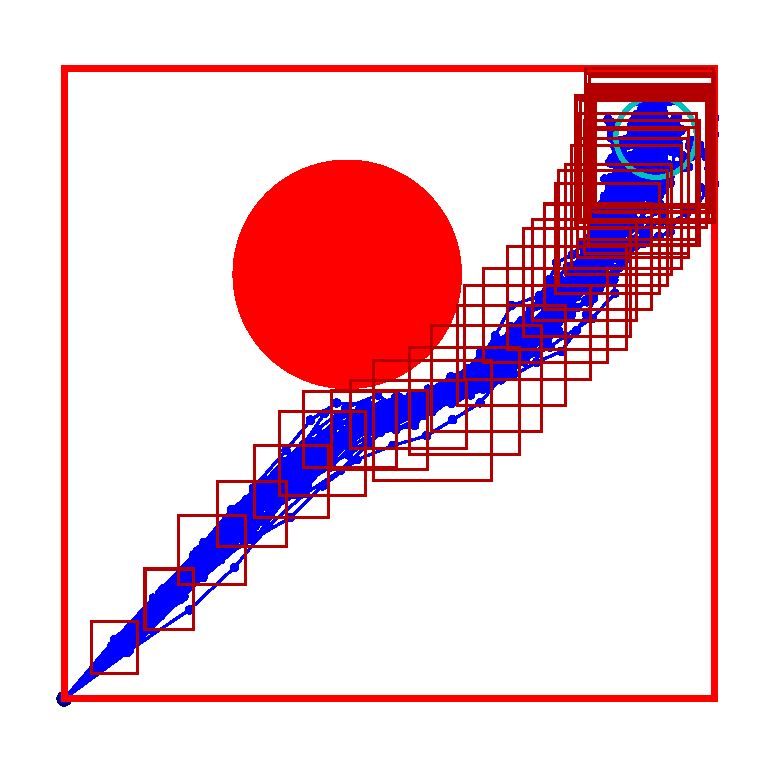
\includegraphics[width=\FS\textwidth]{Codes/BasicsSafety/PessimisticModel40.eps}%
        }%
    \end{figure}
    \textcolor{red}{Illustrate: wide \& thin-tailed distribution requires a big box, to contain transitions that almost surely won't happen. Who does it?}
  \end{overlayarea} 



\end{columns}

%\vspace{-1cm}
  




\end{frame}

%\section{Probabilistic Safety in Decision Making}


\begin{frame}{\normalsize MDPs with probabilistic safety}
\footnotesize

\begin{columns}
\column{0.54\textwidth}
\begin{alertblock}{}
\textbf{In words}
\vspace{-.2cm}
\begin{align*}
\vect\pi^\star = \argmax_{\vect\pi}&\quad\mathrm E\left[ \sum_{\text{time}} \text{Utility}\right]\\
\mathrm{s.t.}&\quad \text{Probability of no violation} \geq c
\end{align*}
\end{alertblock}



\column{0.44\textwidth}
\visible<2->{
\begin{block}{}
\textbf{Formally}
\vspace{-.2cm}
\begin{align*}
\vect\pi^\star = \argmax_{\vect\pi}&\quad\mathrm E\left[ \sum_{k=0}^\infty \gamma^kL\left(\vect s_k,\vect a_k\right)\right]\\
\mathrm{s.t.}&\quad \mathrm{P}\left[ \vect s_{0,\ldots\infty}\in \mathbb S\right] \geq c
\end{align*}
\end{block}}
\end{columns}

\begin{columns}[t]
\column{0.5\textwidth}
\vspace{.5cm}\\
\visible<3->{
\textbf{Remarks}:
\begin{itemize}
%\item Matches the ``worst-case" (robust) version for $c=0$
\item If we can tolerate $c>0$ (small) it can make a big gain in performance
\item Aligned with industrial / practical standards on ``large series"
\item Problem needs a ``termination" (time or goal reached)
\item Building decisions can be difficult from a computational point of view
\end{itemize}}
\column{0.5\textwidth}
\vspace{-.25cm}
 \begin{figure}
   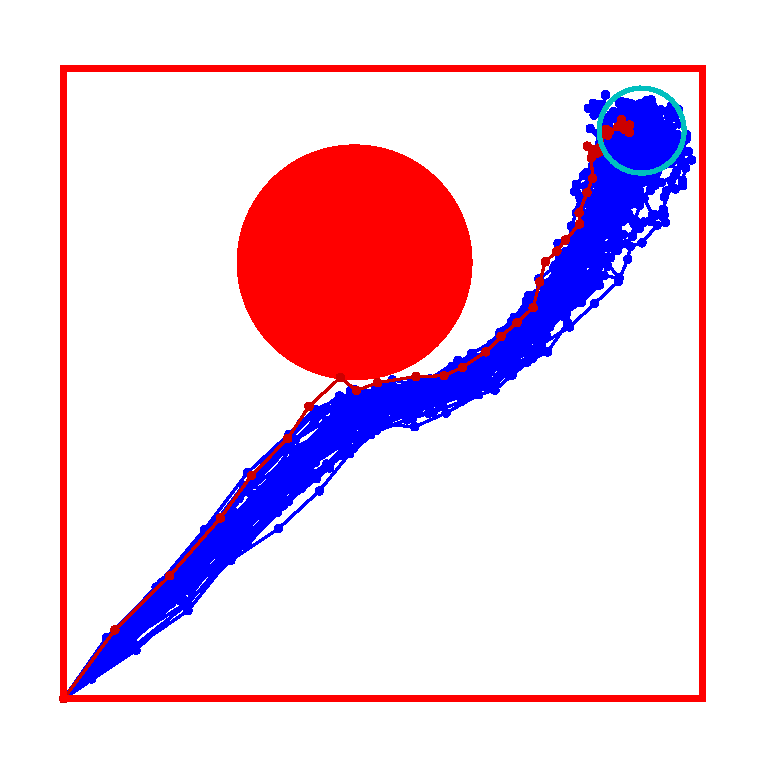
\includegraphics[width=0.98\textwidth]{Codes/BasicsSafety/ProbabilisticModel.eps}%
  \end{figure}
\end{columns}

\end{frame}


\section{Methods}

\begin{frame}{\normalsize Robust Repeated Planning}
\footnotesize
\begin{itemize}
\item Introduction: Robust MPC, Scenario Trees, MC, robust multi-stage stochastic programing, MPPI?
\item Difficulties: guarantees for nonlinear systems, persistent safety (recursive feasibility)
\end{itemize}

\begin{columns}[t]
\column{0.5\textwidth}


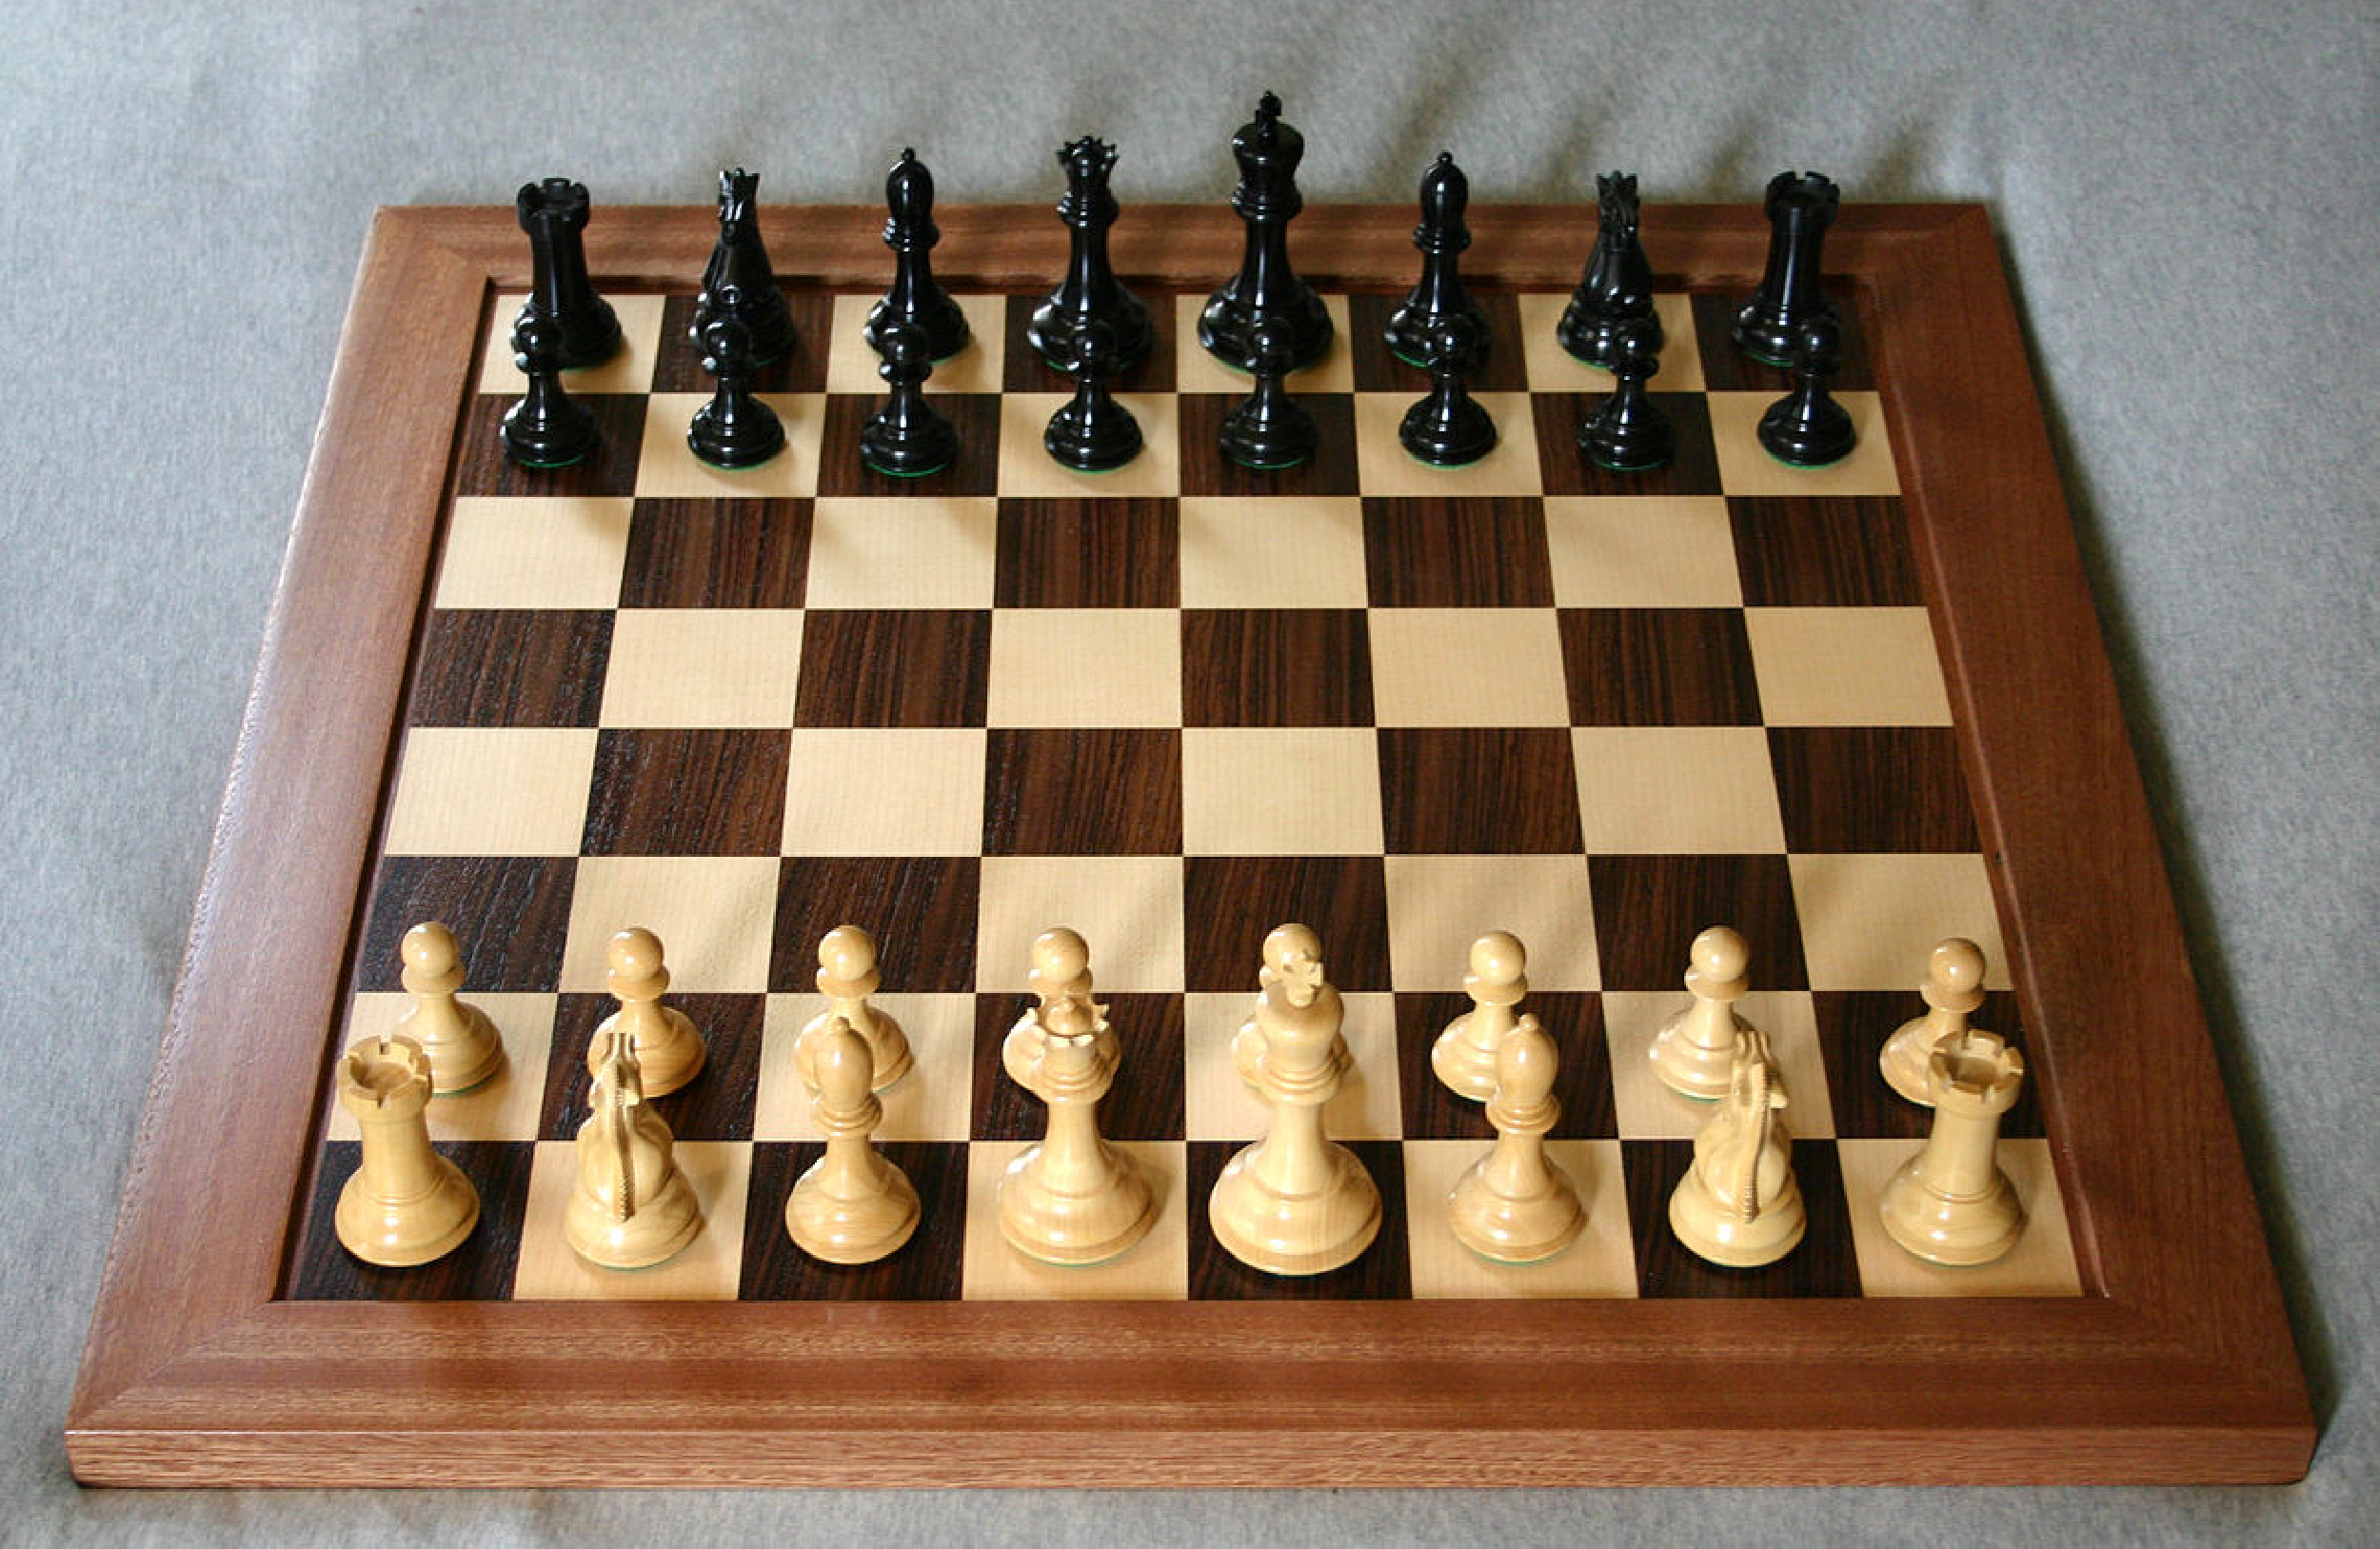
\includegraphics[width=1\textwidth,clip]{Figures/Chess.eps}
\column{0.5\textwidth}
\end{columns}

\end{frame}


\begin{frame}{\normalsize Dynamic Programming \& RL with Probabilistic Safety}
\footnotesize
\begin{columns}[t]
\column{0.65\textwidth}
\begin{columns}[t]
\column{0.1\textwidth}

\column{0.8\textwidth}

\begin{alertblock}{}
\vspace{-.2cm}
\begin{align*}
\vect\pi^\star = \argmax_{\vect\pi}&\quad\mathrm E\left[ \sum_{k=0}^\infty \gamma^kL\left(\vect s_k,\vect a_k\right)\right]\\
\mathrm{s.t.}&\quad \mathrm{P}\left[ \vect s_{0,\ldots\infty}\in \mathbb S\right] \geq c
\end{align*}
\end{alertblock}
\column{0.1\textwidth}
\end{columns}
\begin{block}{}
\textbf{Expected value form} \textcolor{red}{Illustrate??}
\vspace{-.2cm}
\begin{align*}
\vect\pi^\star = \argmax_{\vect\pi}&\quad\mathrm E\left[ \sum_{k=0}^\infty \gamma^kL\left(\vect s_k,\vect a_k\right)\right]\\
\mathrm{s.t.}&\quad \mathrm{E}\left[ \begin{array}{cc}\textcolor{blue}{1}&\text{if no violation occurred}\\\textcolor{myRed}{0}&\text{otherwise}\end{array} \right] \geq c
\end{align*}
\end{block}

\column{0.35\textwidth}
 \begin{figure}
   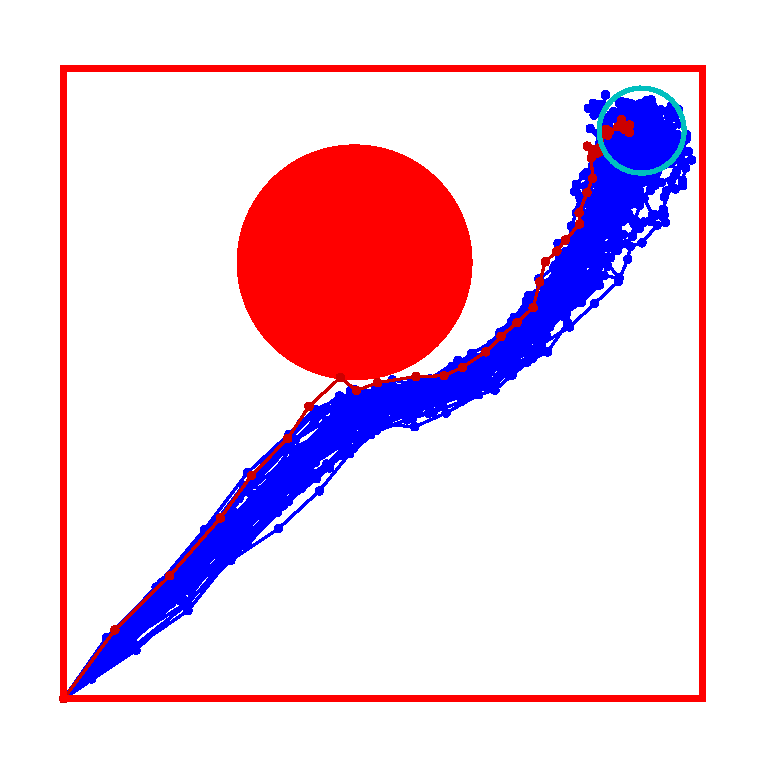
\includegraphics[width=0.98\textwidth]{Codes/BasicsSafety/ProbabilisticModel.eps}%
  \end{figure}
\end{columns}
\begin{itemize}
\item Expected value form enables classical techniques (ref. 1st lecture), i.e. DP and RL
\item Difficulties: estimate expected values (sample based) when $\mathrm{P}\left[ \vect s_{0,\ldots\infty}\in \mathbb S\right]$ is close to 1. \textcolor{red}{Illustrate??}
\end{itemize}


\end{frame}

\begin{frame}{\normalsize Safety Filters \& Reinforcement Learning}
\footnotesize
\begin{itemize}
\item For any state $\vect s$, an ``oracle" tells you which actions will not jeopardize safety in the long run$\rightarrow$``Safe set" $\mathrm{S}\left(\vect s\right)$
\item \visible<2->{We can learn an ``unsafe" policy $$\vect\pi^\star = \argmax_{\vect\pi}\quad\mathrm E\left[ \sum_{\text{time}} \text{Utility}\right]$$
\begin{flushright} that focuses only on utility\end{flushright}}
\item \visible<3->{For state $\vect s$, take the decisions using: $\text{Action} = \text{Projection}_{\mathrm{S}(\vect s)}\left[\vect\pi^\star\left(\vect s\right)\right]$}

\end{itemize}

\begin{columns}[t]
\column{0.6\textwidth}

\begin{overlayarea}{\textwidth}{0.3\textheight}
\only<13-14>{
\textbf{Remark}: ``oracle" can be very hard to build, or not...
\begin{columns}[t]
\column{0.5\textwidth}
\visible<13->{
\vspace{-.35cm}
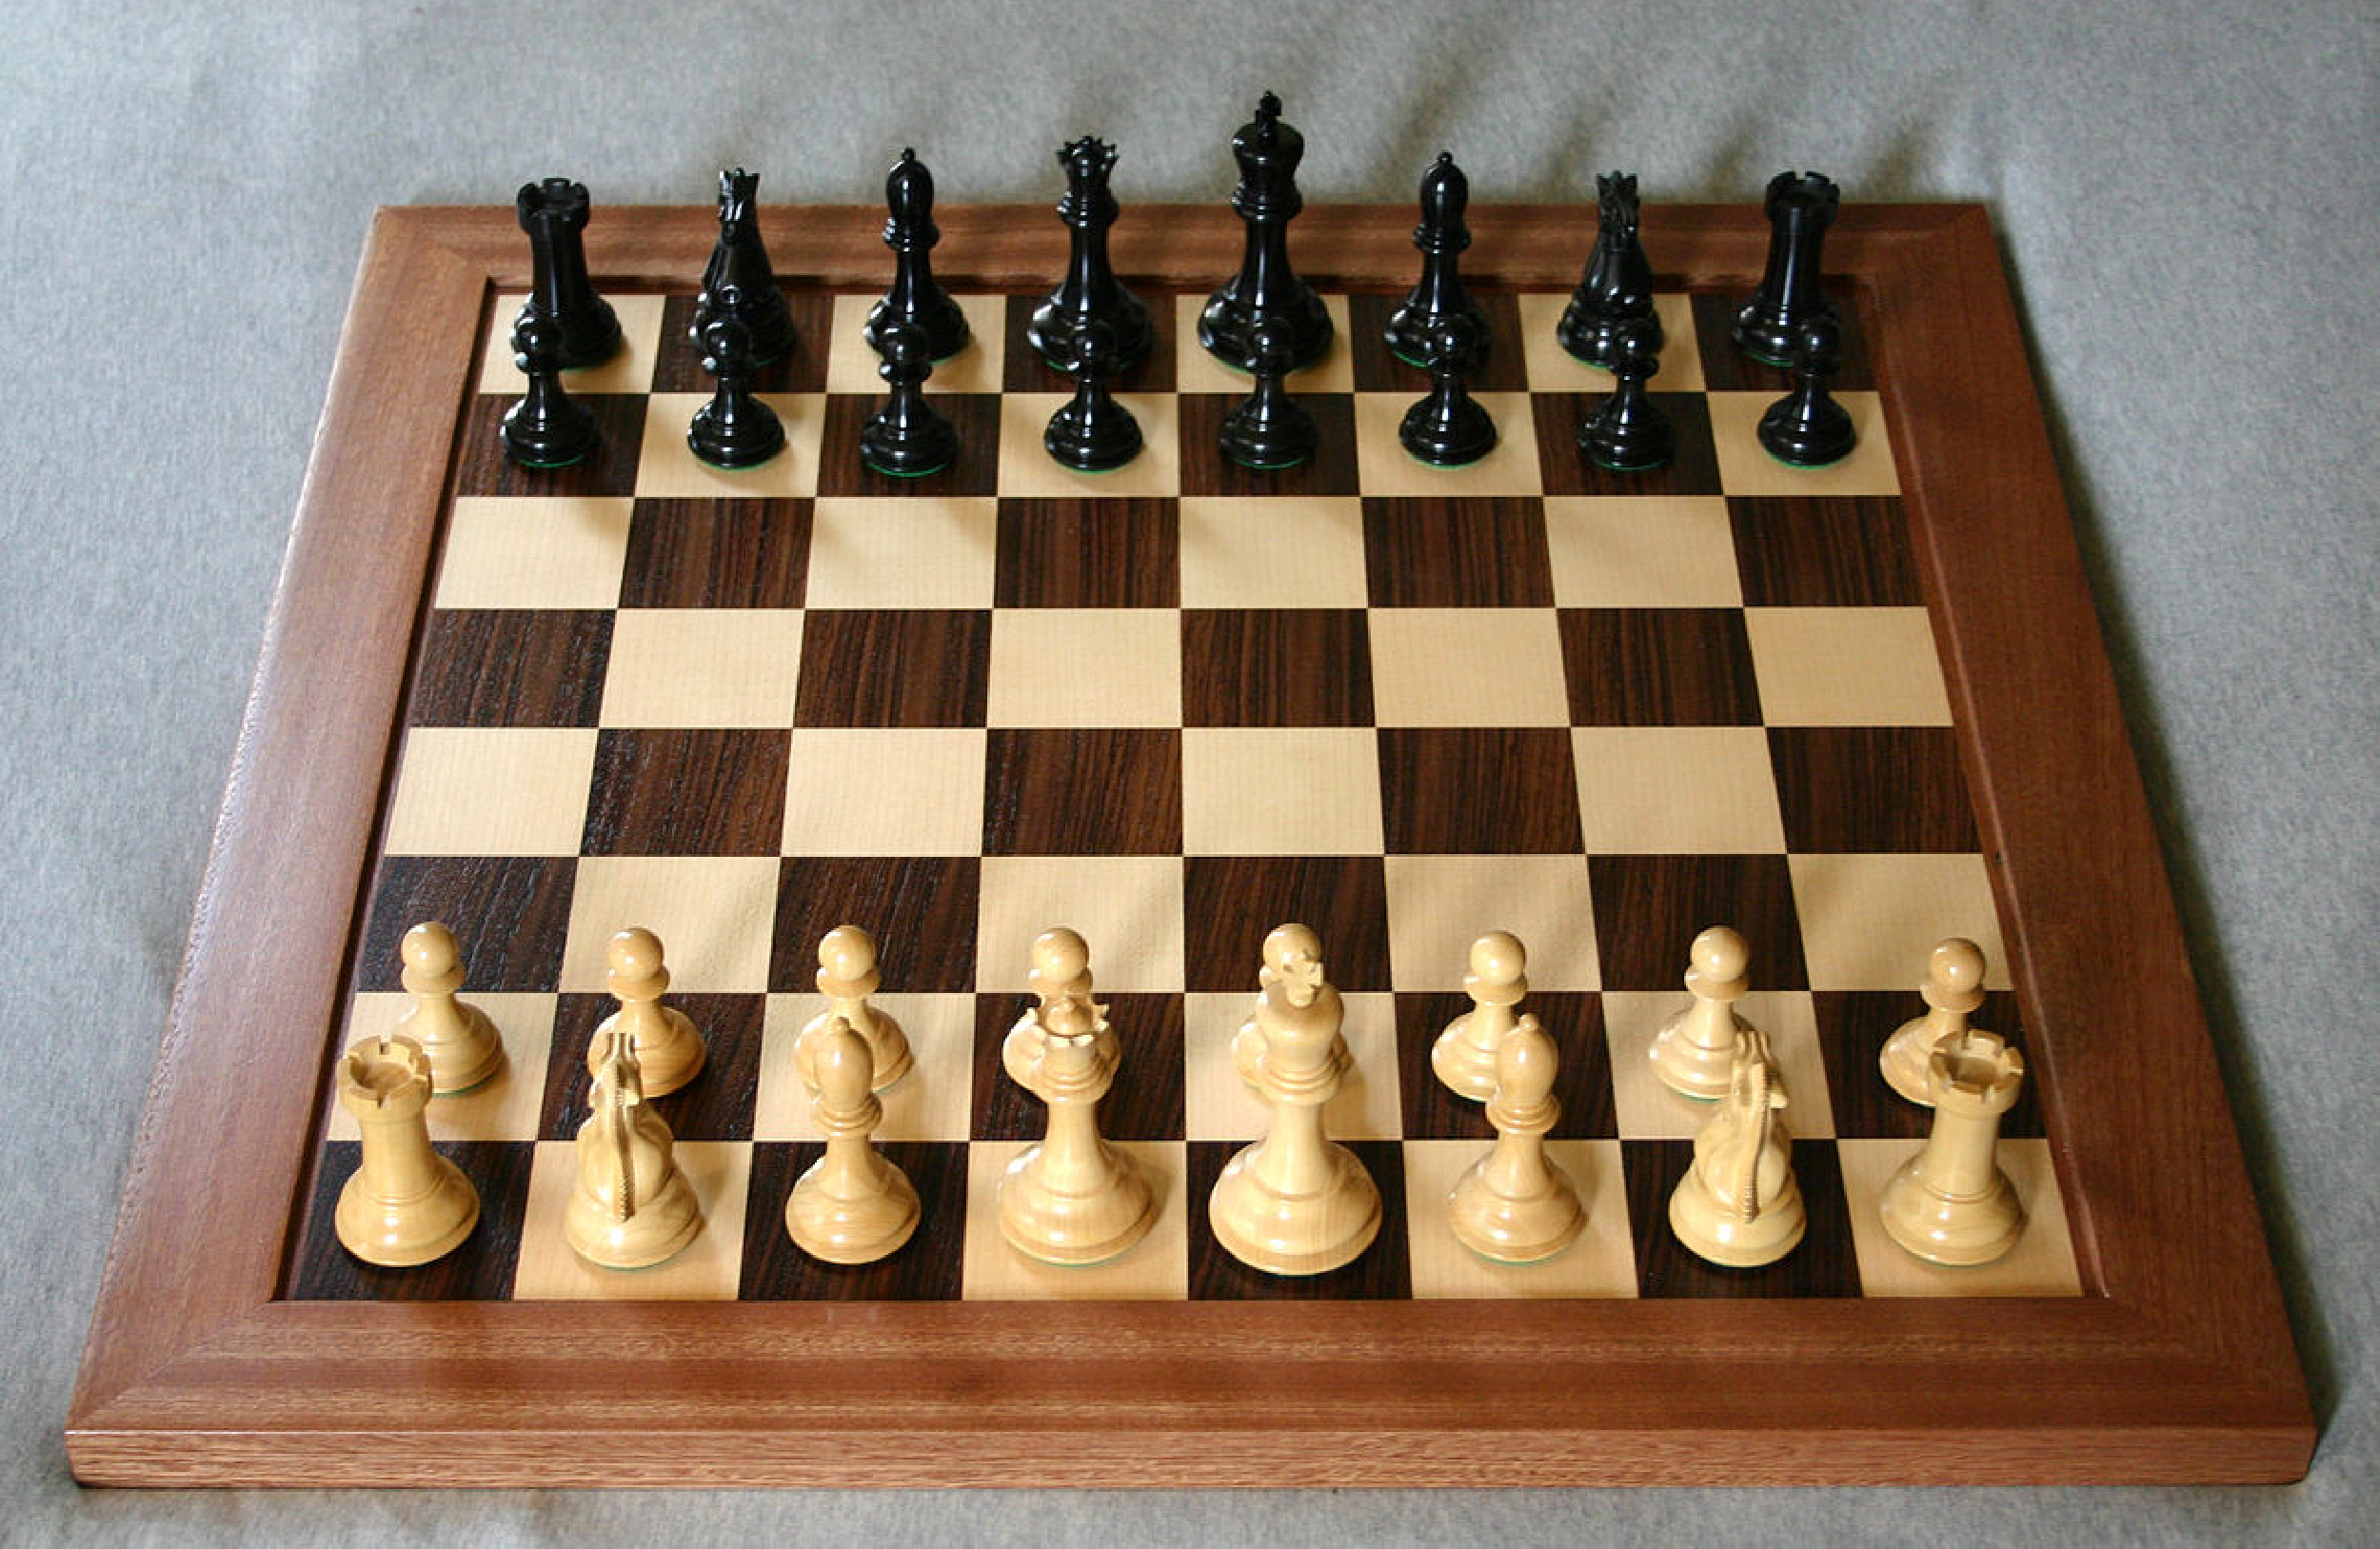
\includegraphics[width=1.025\textwidth,clip]{Figures/Chess.eps}
\center
Not losing the king}
\column{0.5\textwidth}
\visible<14->{
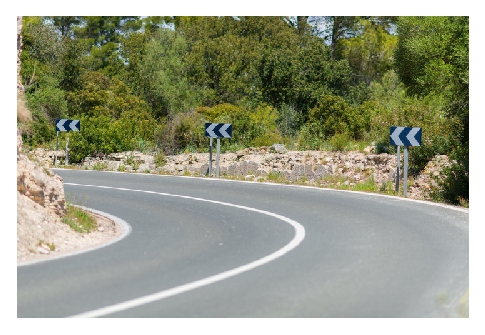
\includegraphics[width=1\textwidth,clip]{Figures/BlindCurve.eps}
\center
\vspace{-.25cm}
Able to stop within the visible distance}
\end{columns}
}
\only<15>{
\textbf{Remarks}:
\begin{itemize}
\item Often close to practice, e.g., flight envelop protection in modern airplane, semi-autonomous driving in cars, etc
\item Oracle $\Rightarrow$ knowledge-based \& conservative!
\end{itemize} 
}
\end{overlayarea}


%\visible<13-14>{\textbf{Remarks}: the ``oracle" can be very hard to build, or not...}
%\begin{columns}[t]
%\column{0.6\textwidth}
%\visible<13->{
%\begin{columns}
%\column{0.5\textwidth}
%\vspace{-.35cm}
%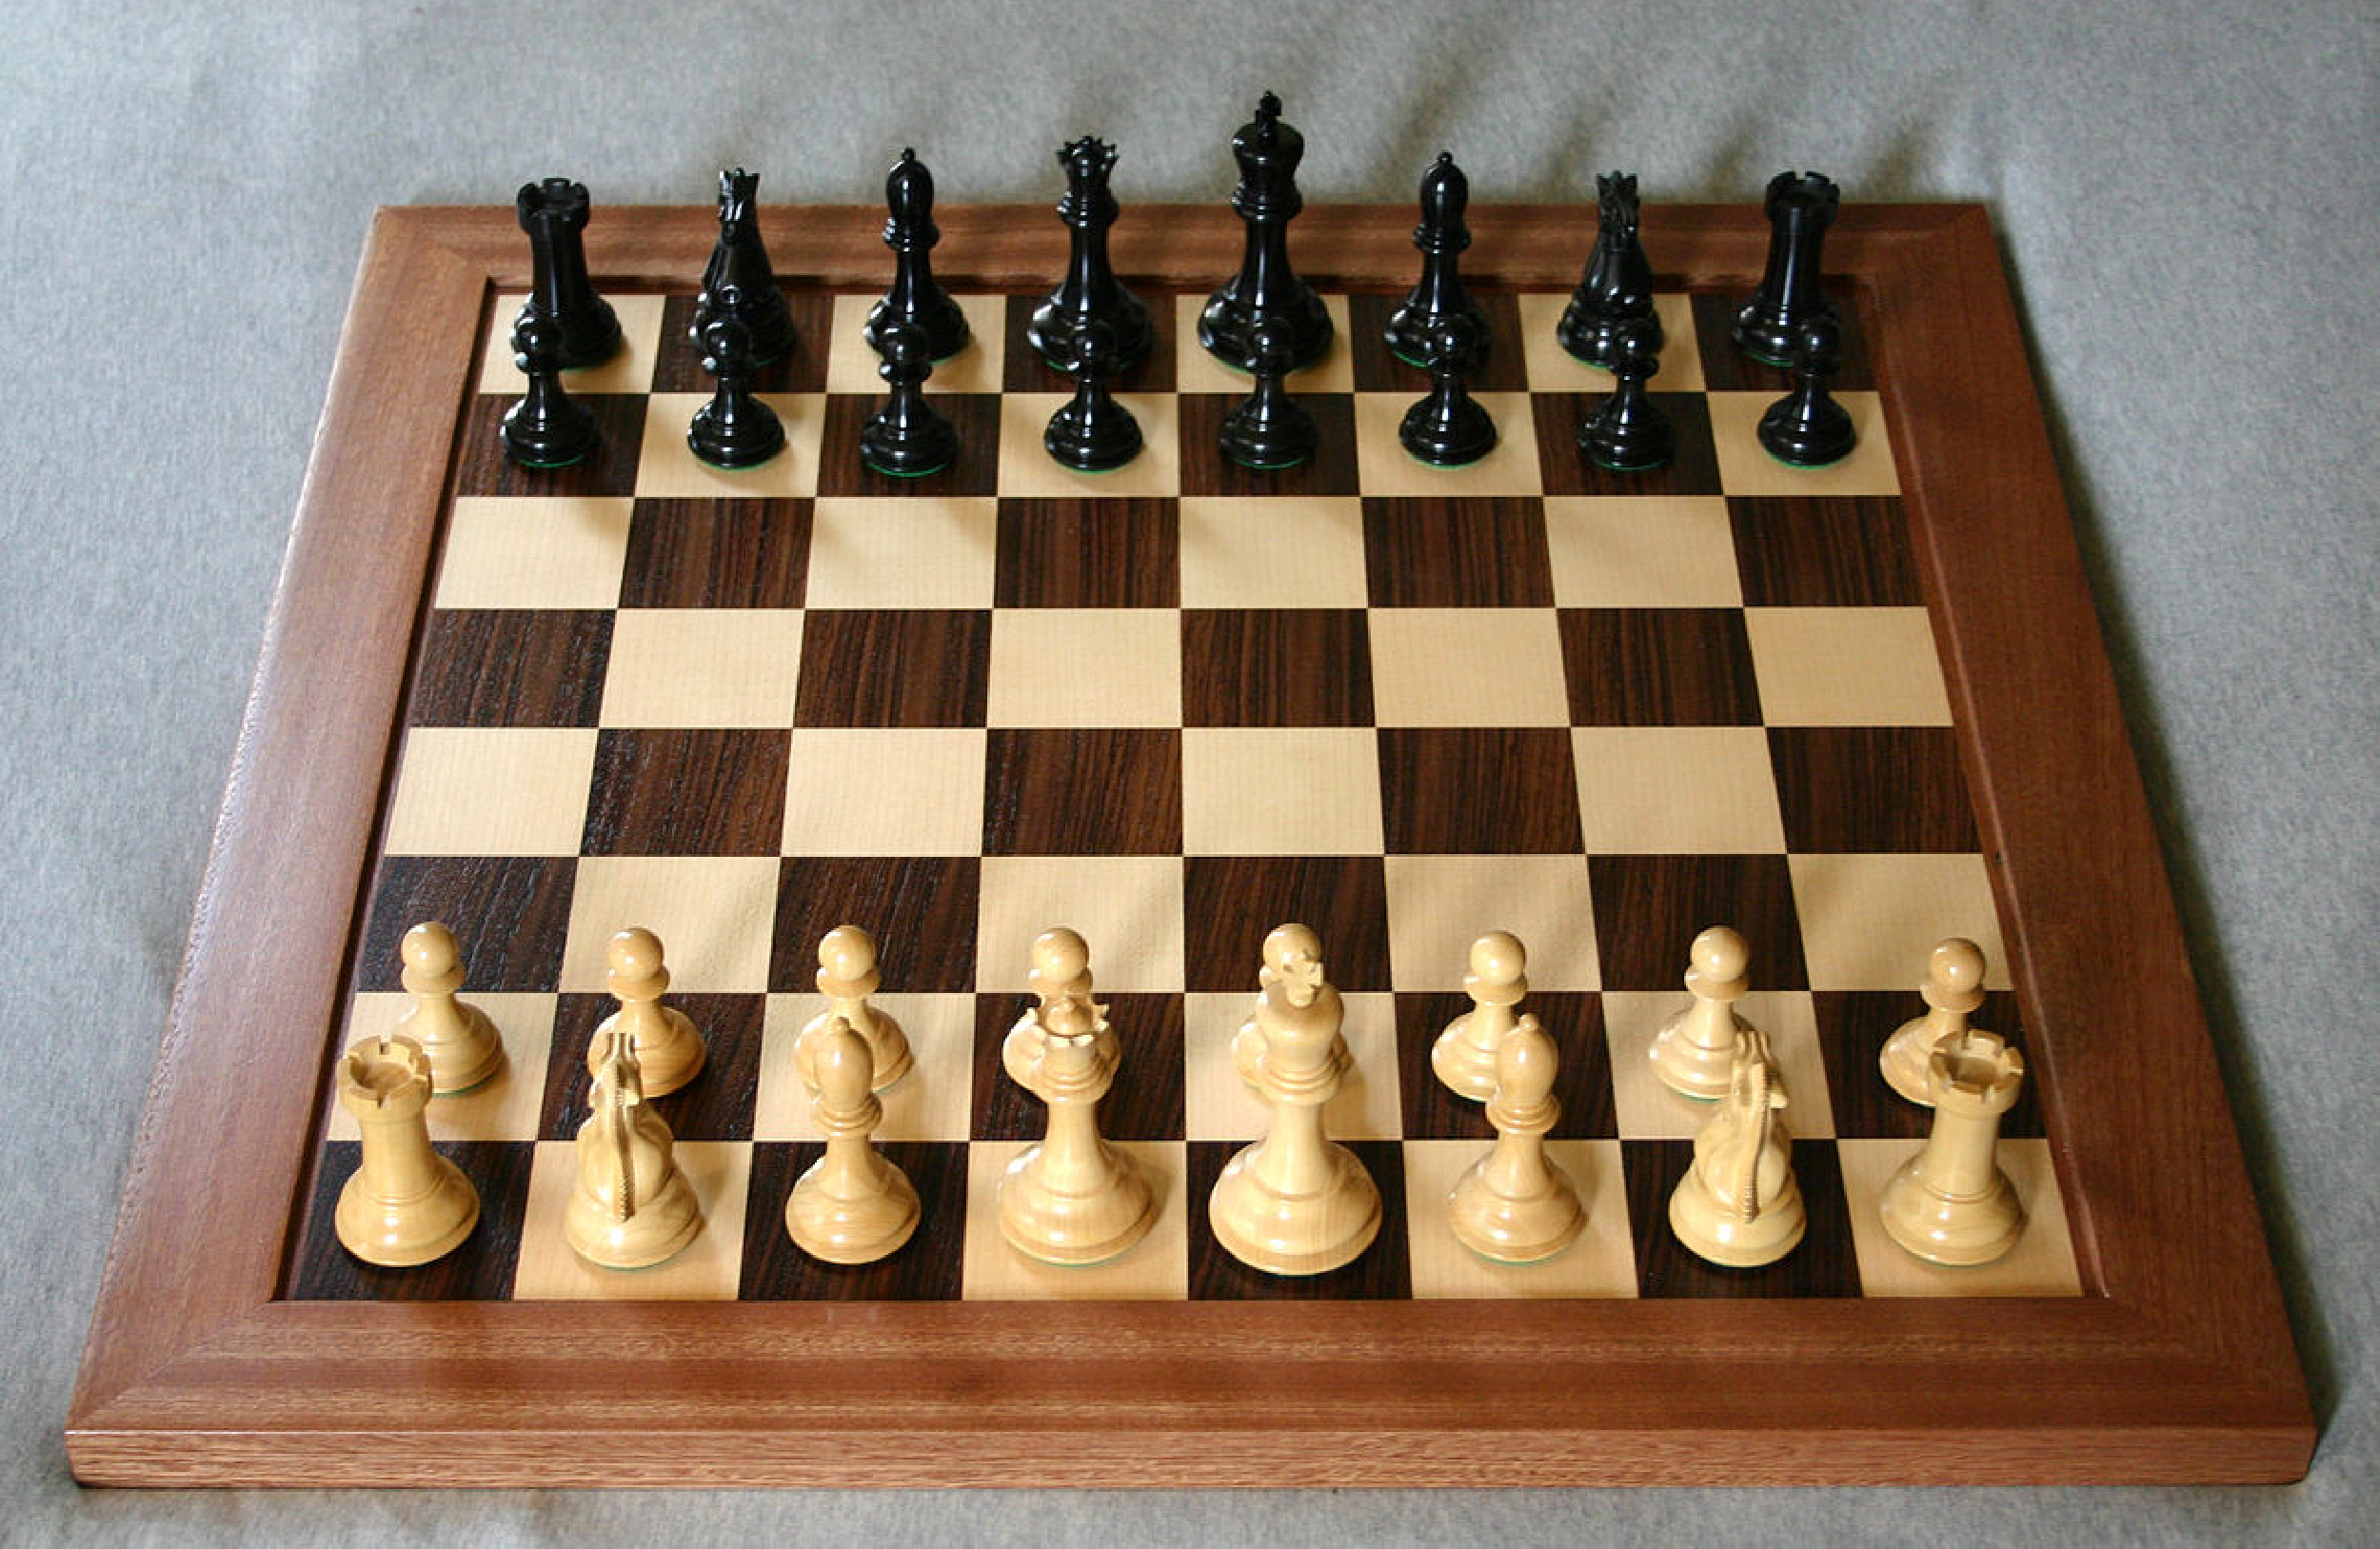
\includegraphics[width=1.05\textwidth,clip]{Figures/Chess.eps}
%\center
%Not losing the king
%\column{0.5\textwidth}
%\visible<14->{
%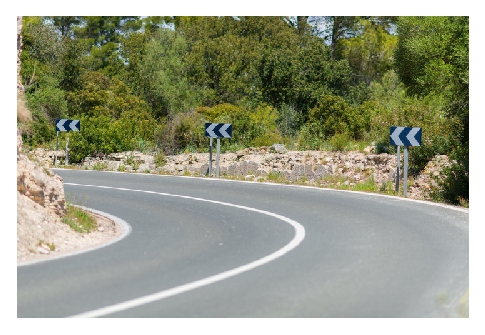
\includegraphics[width=1\textwidth,clip]{Figures/BlindCurve.eps}
%\center
%Able to stop within the visible distance}
%\end{columns}}

\column{0.3\textwidth}

  \begin{overlayarea}{\textwidth}{.5\textheight}
    \begin{figure}
     \newcommand{\FS}{1}
      \only<3>
        {
        \center
	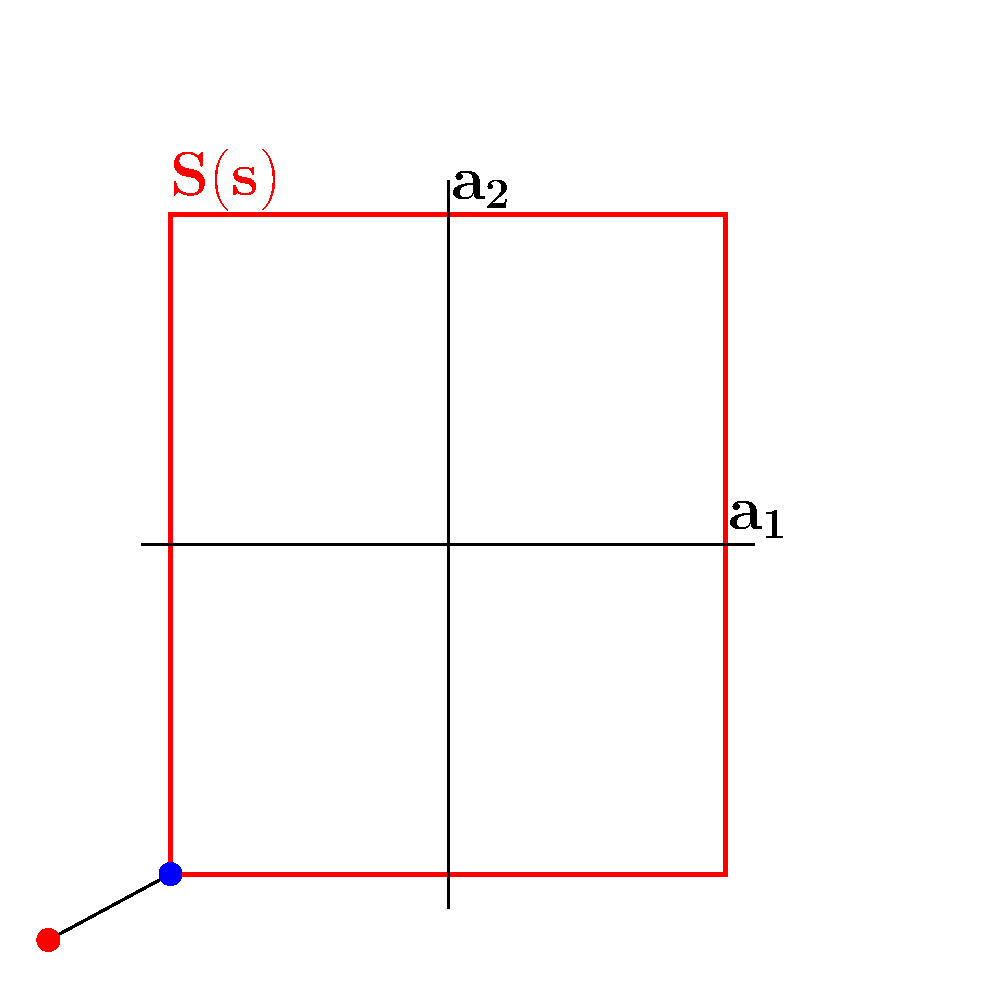
\includegraphics[width=1\textwidth,clip]{Codes/SafetyFilters/Projection0.eps}
	}
	      \only<4>
        {
        \center
	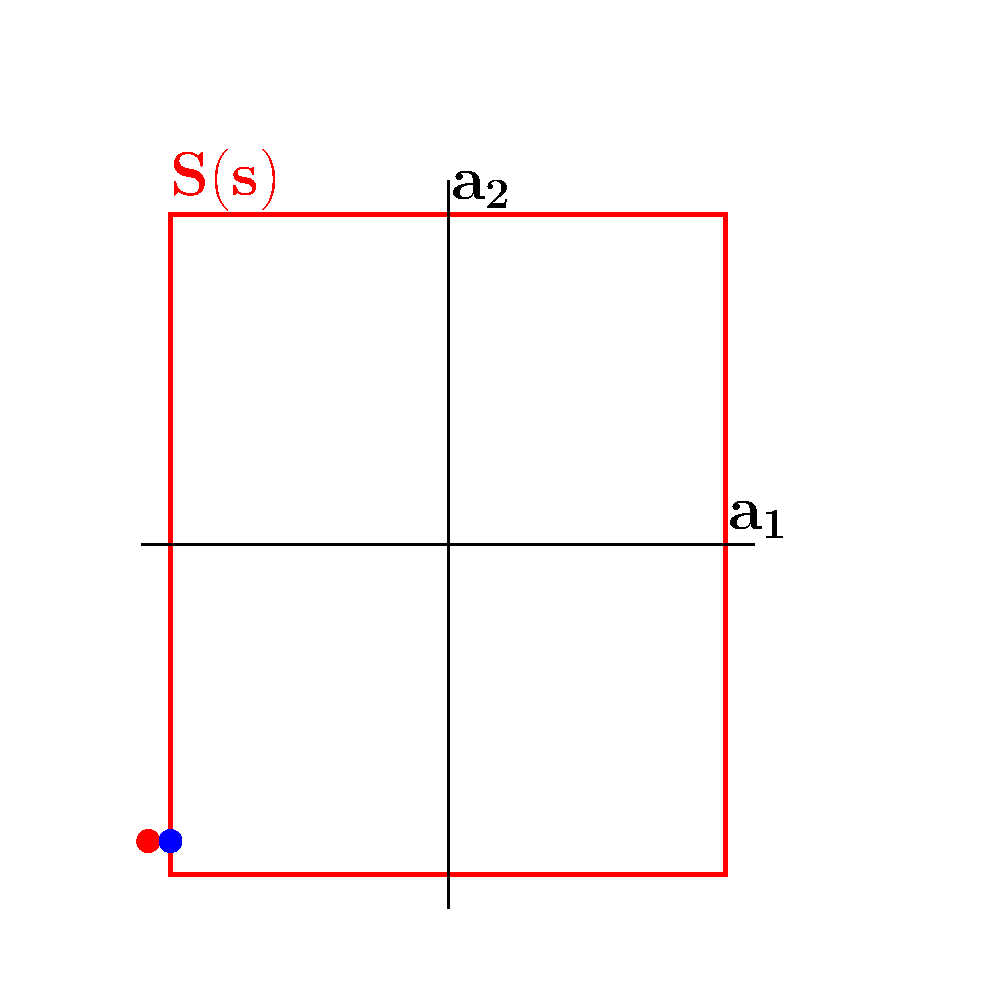
\includegraphics[width=1\textwidth,clip]{Codes/SafetyFilters/Projection1.eps}
	}
	      \only<5>
        {
        \center
	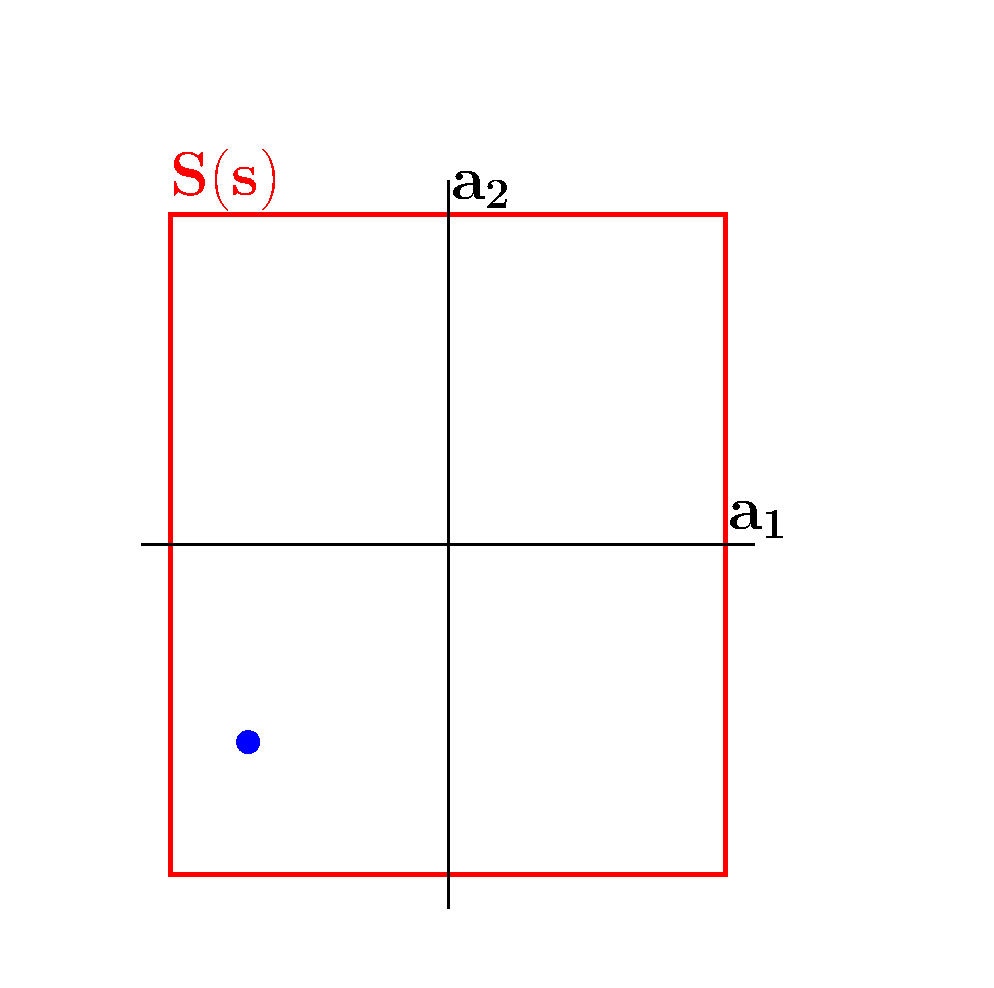
\includegraphics[width=1\textwidth,clip]{Codes/SafetyFilters/Projection2.eps}
	}
	      \only<6>
        {
        \center
	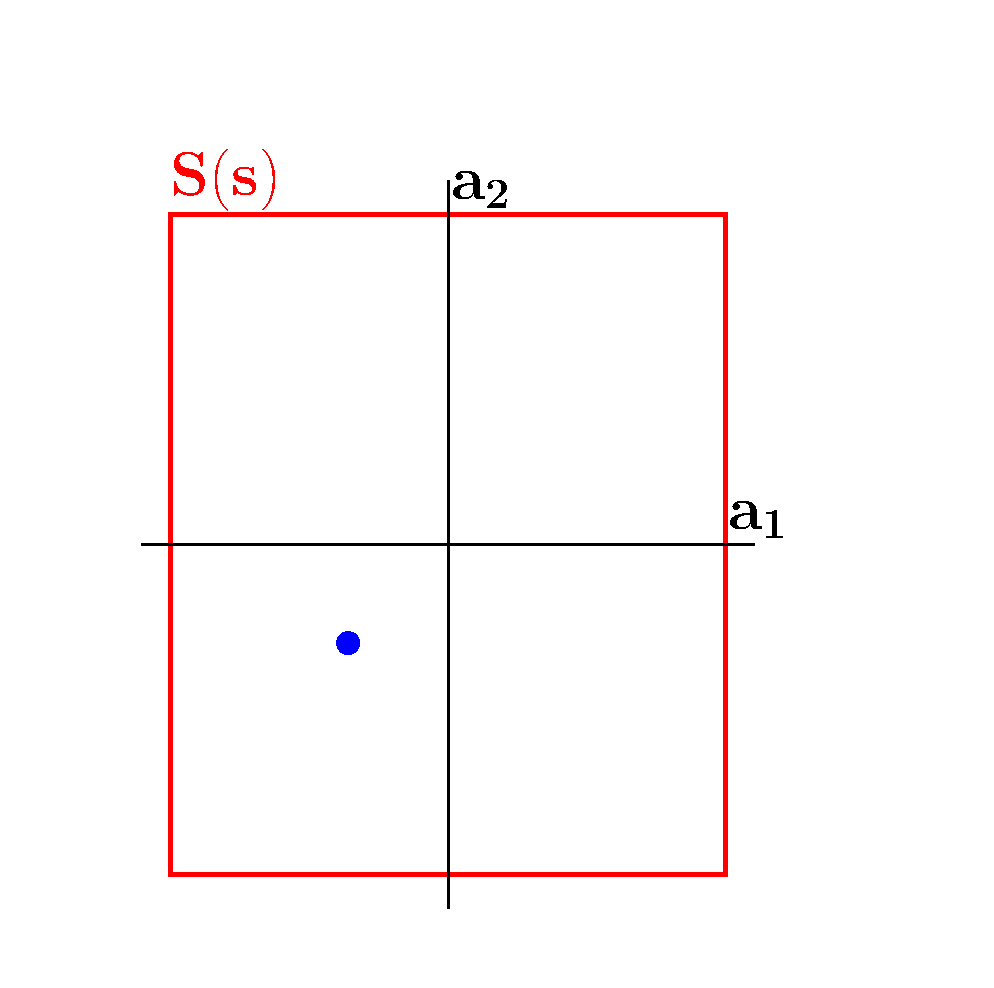
\includegraphics[width=1\textwidth,clip]{Codes/SafetyFilters/Projection3.eps}
	}
	      \only<7>
        {
        \center
	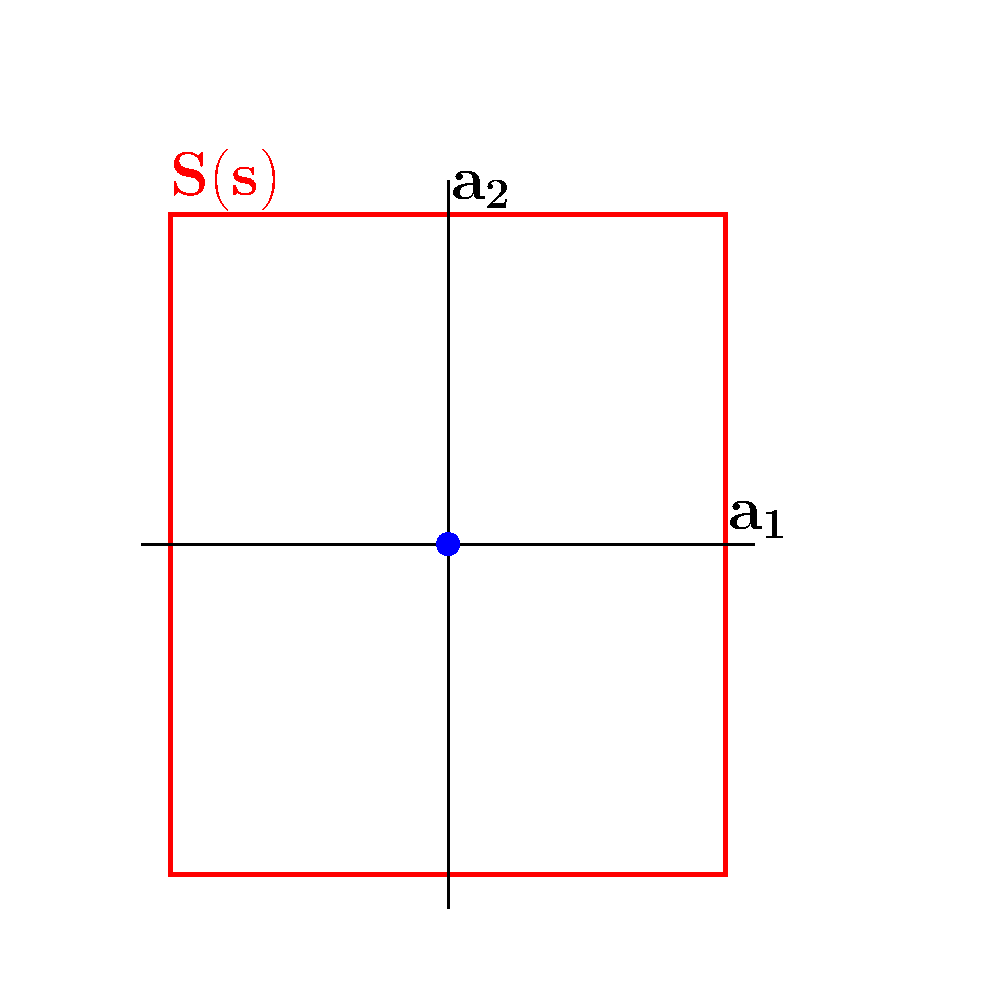
\includegraphics[width=1\textwidth,clip]{Codes/SafetyFilters/Projection4.eps}
	}
	      \only<8>
        {
        \center
	\includegraphics[width=1\textwidth,clip]{Codes/SafetyFilters/Projection5.eps}
	}
	      \only<9>
        {
        \center
	\includegraphics[width=1\textwidth,clip]{Codes/SafetyFilters/Projection6.eps}
	}
	      \only<10>
        {
        \center
	\includegraphics[width=1\textwidth,clip]{Codes/SafetyFilters/Projection7.eps}
	}
	      \only<11>
        {
        \center
	\includegraphics[width=1\textwidth,clip]{Codes/SafetyFilters/Projection8.eps}
	}
	      \only<12->
        {
        \center
	\includegraphics[width=1\textwidth,clip]{Codes/SafetyFilters/Projection9.eps}
	}
%		      \only<14->
%        {
%        \center
%	\includegraphics[width=1\textwidth,clip]{Figures/Chess.eps}
%	}
\end{figure}
\end{overlayarea}
	
\end{columns}

\end{frame}




\begin{frame}{\normalsize Control Barrier Functions (CBFs)}
\begingroup
% Tighter look + small headers
\setbeamerfont{block title}{size=\small}
\scriptsize
% Visible gap between the "In words" and "Formally" columns
\setlength{\columnsep}{1.1cm}

% =======================
% TOP HALF: text content
% =======================
\begin{columns}[T,onlytextwidth]
  % ---- Left: In words (always visible) ----
  \column{0.45\textwidth}
  \begin{alertblock}{}
  \textbf{In words}
  \vspace{-0.25em}
  \begin{itemize}
    \item CBFs provide a formal, model-based way to build the ``oracle'' safe set.
    \item Use a barrier function $h(x)$ so that staying safe means $h(x)\ge 0$.
    \item At each step, if the proposed action would leave the safe set, a small QP minimally adjusts it be safe.
  \end{itemize}
  \vspace{-0.35em}
  \end{alertblock}

  % ---- Right: Formal (appears from overlay 2) ----
  \column{0.48\textwidth}
  \only<2->{
  \begin{block}{}
    \textbf{Formally}
  \vspace{-0.3em}
  \[ 
  \dot x = f(x)+g(x)u,\qquad \mathcal{C}=\{x: h(x)\ge 0\}
  \]
  % \vspace{-0.6em}
  \[
    u^\star(x) = \arg\min_{u}\tfrac12\|u-u_{\mathrm{des}}(x)\|_2^2
    \quad\text{s.t.}
  \]
    \[
  \quad\underbrace{L_f h(x) + L_g h(x)\,u + \alpha(h(x)) \ge 0}_{\text{\scriptsize CBF constraint}}
  \]
  \vspace{-0.6em}
  \end{block}
  } % end only<2->
\end{columns}

\vspace{0.4em}

% =======================
% BOTTOM HALF: figures
% =======================
\begin{columns}[T,onlytextwidth]
  % ---- Left figure: swap unsafe -> safe on overlay 4 ----
  \column{0.52\textwidth}
  % Fix the drawing area so later content doesn't reflow
  \begin{overlayarea}{\linewidth}{0.42\textheight}
    \only<1-3>{
      \begin{figure}
        \centering
        \includegraphics[width=0.40\linewidth]{Codes/CBF/CBF_Traj_unsafe.eps}
        \caption*{\scriptsize Unsafe trajectory: violates $h(x)\ge 0$.}
      \end{figure}
    }% end only<1-3>
    \only<4>{
      \begin{figure}
        \centering
        \includegraphics[width=0.4\linewidth]{Codes/CBF/CBF_Traj_safe.eps}
        \caption*{\scriptsize CBF-filtered trajectory.}
      \end{figure}
    }% end only<4>
  \end{overlayarea}

  % ---- Right figure: QP projection appears from overlay 3 ----
  \column{0.48\textwidth}
  \begin{overlayarea}{\linewidth}{0.42\textheight}
    \only<1-2>{ % keep the area blank on overlays 1-2 to preserve layout
      \vspace{0.2em}
    }
    \only<3->{
      \begin{figure}
        \centering
        \includegraphics[width=0.55\linewidth]{Codes/CBF/CBF_QP_projection.eps}
        \caption*{\scriptsize CBF filter: project $u_{\mathrm{des}}$ to feasible $u_{\mathrm{safe}}$.}
      \end{figure}
    }
  \end{overlayarea}
\end{columns}

% ==============
% remarks 
% ==============
\only<4->{%
\vspace{-0.35em}
\scriptsize
\begin{itemize}
  \item The barrier function and safe set $\mathcal{C}$ are typically \textbf{constructed from domain knowledge} (physics, rules, safety envelopes).
  \item Requires a (possibly simplified, conservative) \textbf{system model}: \textbf{robust} approach.
\end{itemize}
}

\endgroup

\end{frame}

\section{Safe Decisions from Data \& AI}

\begin{frame}{\normalsize Reinforcement Learning with Safety}
\footnotesize

\textcolor{red}{SG can do}

\end{frame}

\section{Epistemic Uncertainty and Safe Decisions}

\begin{frame}{\normalsize The Role of Probabilistic AI}
\footnotesize

\begin{columns}[t]
\column{0.5\textwidth}


  \begin{overlayarea}{\textwidth}{.5\textheight}
    \begin{figure}
     \newcommand{\FS}{1}
      \only<1>
        {
        \center
	\includegraphics[width=1\textwidth,clip]{Codes/Epistemic/DataVsDist0.eps}
	}
	      \only<2>
        {
        \center
	\includegraphics[width=1\textwidth,clip]{Codes/Epistemic/DataVsDist1.eps}
	}
	      \only<3>
        {
        \center
	\includegraphics[width=1\textwidth,clip]{Codes/Epistemic/DataVsDist2.eps}
	}
	      \only<4>
        {
        \center
	\includegraphics[width=1\textwidth,clip]{Codes/Epistemic/DataVsDist3.eps}
	}
	      \only<5->
        {
        \center
	\includegraphics[width=1\textwidth,clip]{Codes/Epistemic/DataVsDist4.eps}
	}
\end{figure}
\end{overlayarea}

\column{0.5\textwidth}
\end{columns}


\end{frame}

\end{document}

\begin{frame}{\normalsize RL over Decision Making}
\footnotesize
\newcommand{\Sys}{\vspace{-0.25cm}\includegraphics[width=1\textwidth,clip]{Figures/SmartHouse.eps}}

%\vspace{-1cm}
\tikzstyle{Sys_block} = [rectangle, draw, fill=none,  text width=3.cm, text centered, rounded corners, minimum height=4em,inner sep=2pt]
\tikzstyle{Obj_block} = [rectangle, draw, fill=myLightRed,  text width=3.2cm, text centered, rounded corners, minimum height=4em,inner sep=2pt]
\tikzstyle{Opt_block} = [rectangle, draw, fill=myLightGreen,  text width=3cm,  text centered, rounded corners]
\tikzstyle{ID_block} = [rectangle, draw, fill=myLightBlue,  text width=3cm, text centered, rounded corners]    

\tikzstyle{RL_block} = [rectangle, draw, fill=none,  text width=3.cm, text centered, rounded corners, minimum height=4em,inner sep=2pt]

\tikzstyle{line} = [draw, -latex']

\begin{tikzpicture}[->,>=stealth']

\node [Sys_block] (sys0) {\Sys};

\node [ID_block, left of=sys0, node distance = 5cm] (ID0) {
 \begin{minipage}[c]{3cm}
% \vspace{-0.2cm}
\textbf{AI model} e.g.
\begin{align*}
\hat{\vect{s}}_{+} \sim \hat{\mathrm P}_{\vect{\theta}}\left[\cdot\,|\,\vect{s},\vect{a}\right]
\end{align*}
\end{minipage}
 };

\visible<3->{
\node [RL_block, above of=ID0, node distance = 2.0cm] (RL0) {
 \begin{minipage}[c]{3cm}
\textbf{RL} 
\vspace{-.25cm} 
\begin{align*}
\Delta\vect\theta = \alpha\nabla_{\vect\theta} J\left(\vect\pi_{\vect \theta}\right)
\end{align*}
\vspace{-.85cm}
\flushright from real data
\end{minipage}
 };}

 
 \node [Opt_block, below of=ID0, node distance = 2.5cm] (opt0) {
 \begin{minipage}[c]{3cm}
 \center
 \center
\textbf{Build Decisions}
\begin{itemize}
\scriptsize
\item Policy
\item Rep. planning
\end{itemize}
\end{minipage}
 };
 
 \node [Obj_block, left of=opt0, node distance = 4cm] (Obj0) {
 \begin{minipage}[c]{3.2cm}
 \center
\textbf{Utility \& Constraints}
\vspace{-.5cm}
\begin{overlayarea}{\textwidth}{0.1\textheight}
\only<1-3>{
\vspace{-.5cm}
\begin{align*}
L\left(\vect s,\vect a\right)
\end{align*}
}
\only<4->{
\vspace{-.5cm}
\begin{align*}
L_{\vect \theta}\left(\vect s,\vect a\right)
\end{align*}
}
\end{overlayarea}

\end{minipage}
 };

\visible<5->{
 \node [Obj_block, left of=RL0, node distance = 4cm] (Obj1) {
 \begin{minipage}[c]{3.2cm}
 \center
\textbf{Utility \& Constraints}
\vspace{-.25cm}
\begin{align*}
L\left(\vect s,\vect a\right)
\end{align*}
\end{minipage}
 };
}

 
 \path 
 (sys0) edge  node[anchor=center,xshift=-.5em] {
  \begin{minipage}[c]{1cm}
  \center
 Data\\ knowledge
 \end{minipage}} (ID0)
 (ID0) edge[bend left=20]  node[anchor=west] {Predictions} (opt0)
 (opt0) edge[bend left=20]  node[anchor=east] {Actions} (ID0)
 (opt0) edge[bend right=20]  node[anchor=west,xshift=1em] {Policy or actions} (sys0)
 (Obj0) edge  node[anchor=south] {} (opt0)
 ;
 
 \visible<3->{
 \path   (sys0) edge[bend right=20]  node[anchor=south west] {
  \begin{minipage}[c]{1cm}
  \center
 Data\\ knowledge
 \end{minipage}} (RL0)
  (RL0) edge  node[anchor=west] {$\Delta\vect\theta$} (ID0);}

 \visible<4->{\path    (RL0) edge[bend right=20]  node[anchor=south east] {$\Delta\vect\theta$} (Obj0);}
 \visible<5->{\path    (Obj1) edge[]  node[anchor=south east] {} (RL0);}


\visible<2->{\draw[blue,thick] ($(ID0.north east)+(+0.15,0.15)$)  rectangle ($(Obj0.south west)+(-0.15,-0.3)$);}
\end{tikzpicture}
\vspace{-.25cm}
\begin{itemize}
\item The model is not $\hat{\mathrm P}_{\vect \theta}$, it is the entire ``decision box"
\item Utility \& Constraints to build decisions from the predictions are part of the model
\item RL can tune the whole \textcolor{blue}{decision box}, from real data + true Utility \& Constraints 
\end{itemize}




\end{frame}


\end{document}

